\section{Performance Evaluation}
\label{sec:results}

In this section we describe the experimental evaluation of the strategy proposed to redirect the users, including the scenarios, metrics, methodology and outcomes.


\subsection{QoE Metric evaluation}

There exist many viewer QoE models in the literature. we will describe the QoE metrics used to score the user satisfaction. Firstly, We compute each video quality chunk by a logarithmic law over bit-rates. Study in~ propose a video quality model for DASH as shown in Equation (1). Each video has $N$ chunks and is encoded with $L$ bitrate levels. $r_i$ represents a specific bitrate level. At each step $i$, the quality of chunk $i$ which is encoded at $l_i$ is defined as:

$$
q(r_i) = a_1 * log(a_2 * (r_i/ r_{|L|}))
$$

To quantify a long-term users' QoE, we require a flexible QoE model that includes the most effective metrics. 
We consider the Eqn. (7) which consists of four metrics: (a) the average chunk perceptual quality, (b) the average number of quality oscillations, (c) the average number of stall events and their durations, and (d) the startup delay. K

\begin{equation}\label{qoe-equation}
QoE_i = \alpha_1 + \alpha_2 + \alpha_3 + \alpha_4
\end{equation}


The QoE has a range of 1 to 5. Where the values 1 = bad, 2 = poor, 3 = fair, 4 = good, and 5 = excellent.
 
 
\subsection{Methodology}

We present three approaches to address the methodological problems identified in a edge/cloud multi-tier network for watching a video streaming: cloud-only 

\subsection{Experimental Setup}

%[29] Christian Kreuzberger, Daniel Posch, and Hermann Hellwagner. Amust framework - adaptive multimedia streaming simulation framework for ns-3 and ndnsim, 2016.
%[30] C. Mueller, S. Lederer, J. Poecher, and C. Timmerer. Demo paper: Libdash - an open source software library for the mpeg-dash standard. In 2013 IEEE International Conference on Multimedia and Expo Workshops (ICMEW), pages 1–2, July 2013.
% Per-title encode optimization, 2015. ; accessed 20-novembro-2019.

To implement DASH servers and users that allow adaptive video streaming, we use Adaptive Multimedia Streaming~(AMuSt)~[1]. The AMuSt framework provides a set of applications for producing and consuming adaptable video, based on the DASH standard. DASH functionality is provided by the libdash library~[2], an open source library that provides an interface to the DASH standard. Currently, libdash is the official reference software for the DASH standard. We consider that users are interested in an available video with ten different bit rate representations \{235kbps, 375kbps, 560kbps, 560kbps, 750kbps, 1050kbps, 1750kbps, 2350kbps, 3000kbps, 4300kbps, 5800kbps\}, which are used by Netflix subsets~[3], which are used by Netflix. [31]. Each representation is divided into 2-second segments. Each experiment one time with a video execution time of 1600 seconds~(800 segments). %Figure 3 shows the topology with three levels used in the experiments, each level \{1, 2 and 3\} is represented as a scenario.

%Dash server and the clients allowed to request a multimedia content in DASH format, was used the Adaptive Multimedia Streaming~(AMuSt). The AMust system allow a set o apps to produce and consume the adaptive video, based on Dash pattern. The DASH functionality is provided by the libdash library, an open source library that provides an interface to the DASH standard. Currently, libdash is the reference software official DASH standard.

For sake of simplicity, the cache video used in simulation are already considered deployed in the edge dash nodes.
We simulate the scenario in a binary tree topology of height two. Firstly, We compare with the cloud-only scenario, without edge cache, to the difference with and without the edge use.

The AP nodes is implemented on an wireless device which communicates via IEEE 802.11g in 2.4GHz frequency. The APs are connected with the routes by a wire and the end-users via wireless. Each users is located exatcly 8 meters of distance.

%To illustrate the idea, we assume tree topology. According to the guideline, a mobile backhaul network is modeled as a two-level hierarchical network. Wireless base stations are connected to aggregation nodes, e.g., service/packet data network gateway (S/P-GW) nodes. Furthermore, aggregation nodes are connected to core nodes, e.g., central office nodes. To the best of our knowledge, separation of traffic from one wireless base stations to multiple aggregation nodes, and from one aggregation node to multiple core nodes is not dominant in current mobile backhaul networks. Thus, we assume a tree-topology backhaul network



% \begin{figure*}
%     \centering
%     \subfigure[]{
%     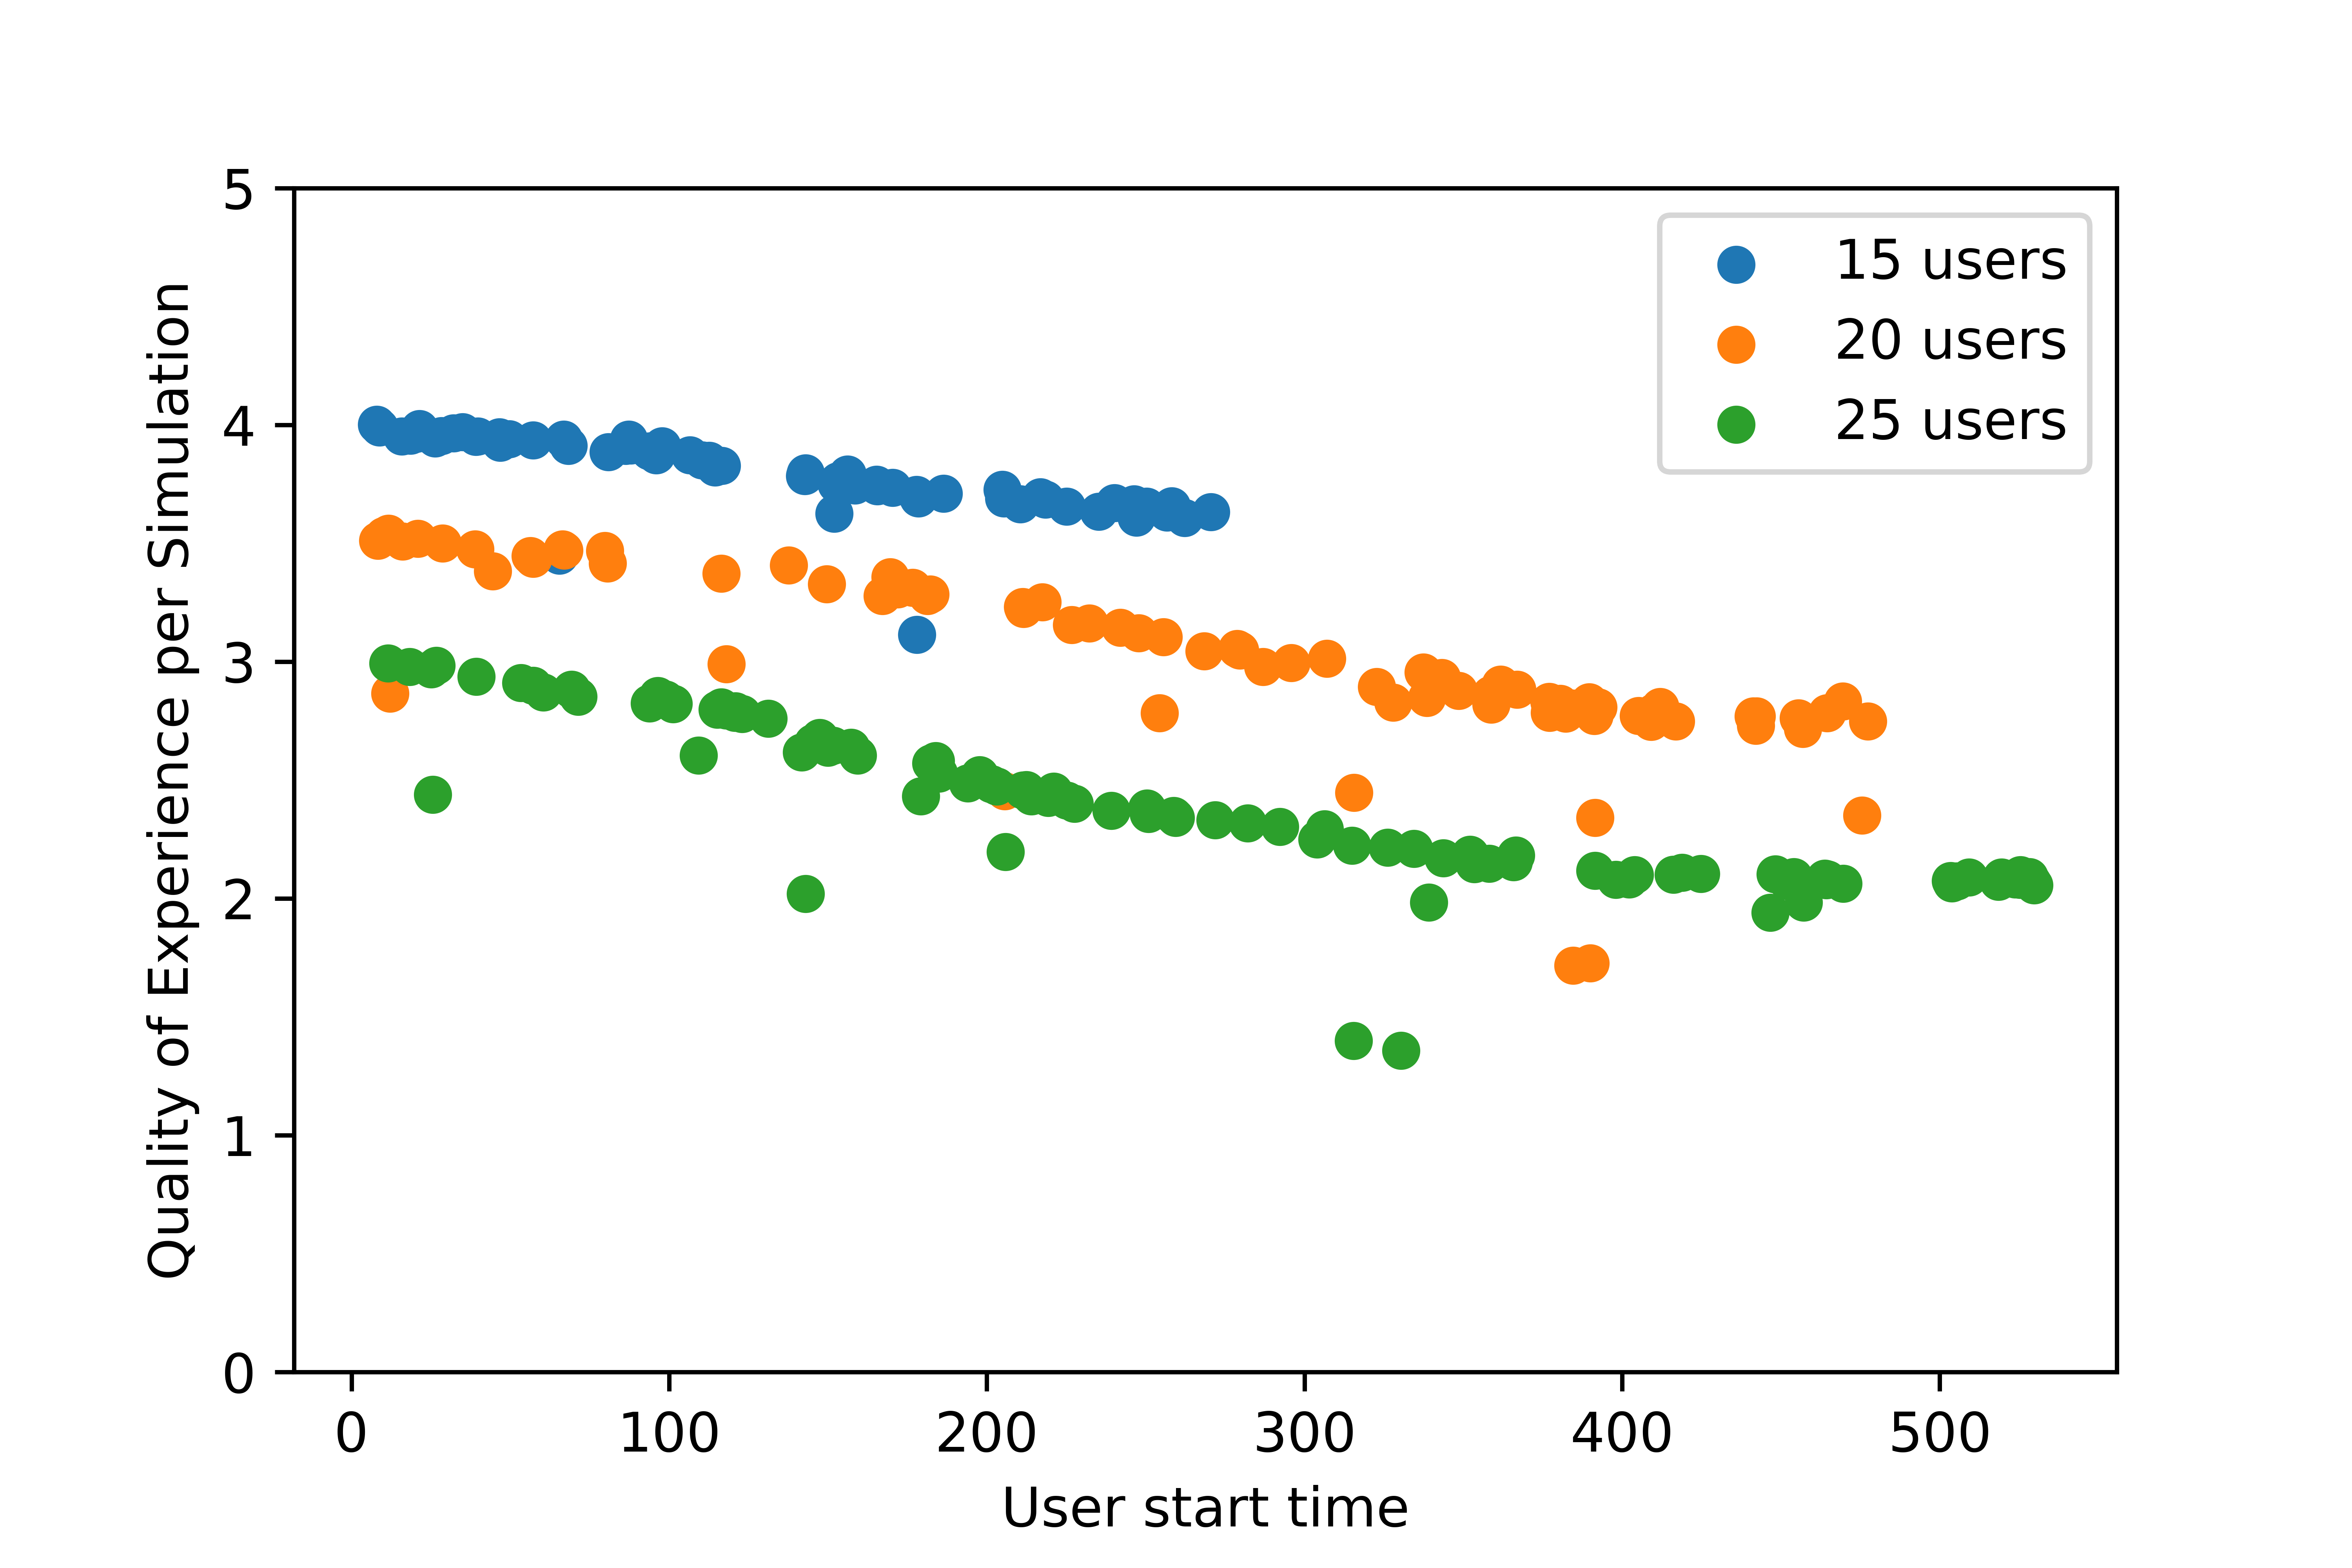
\includegraphics[width=0.45\linewidth]{images/QoECompare.png}
%     \label{fig:red-comparison-plot}
%     }
%     \subfigure[]{
%     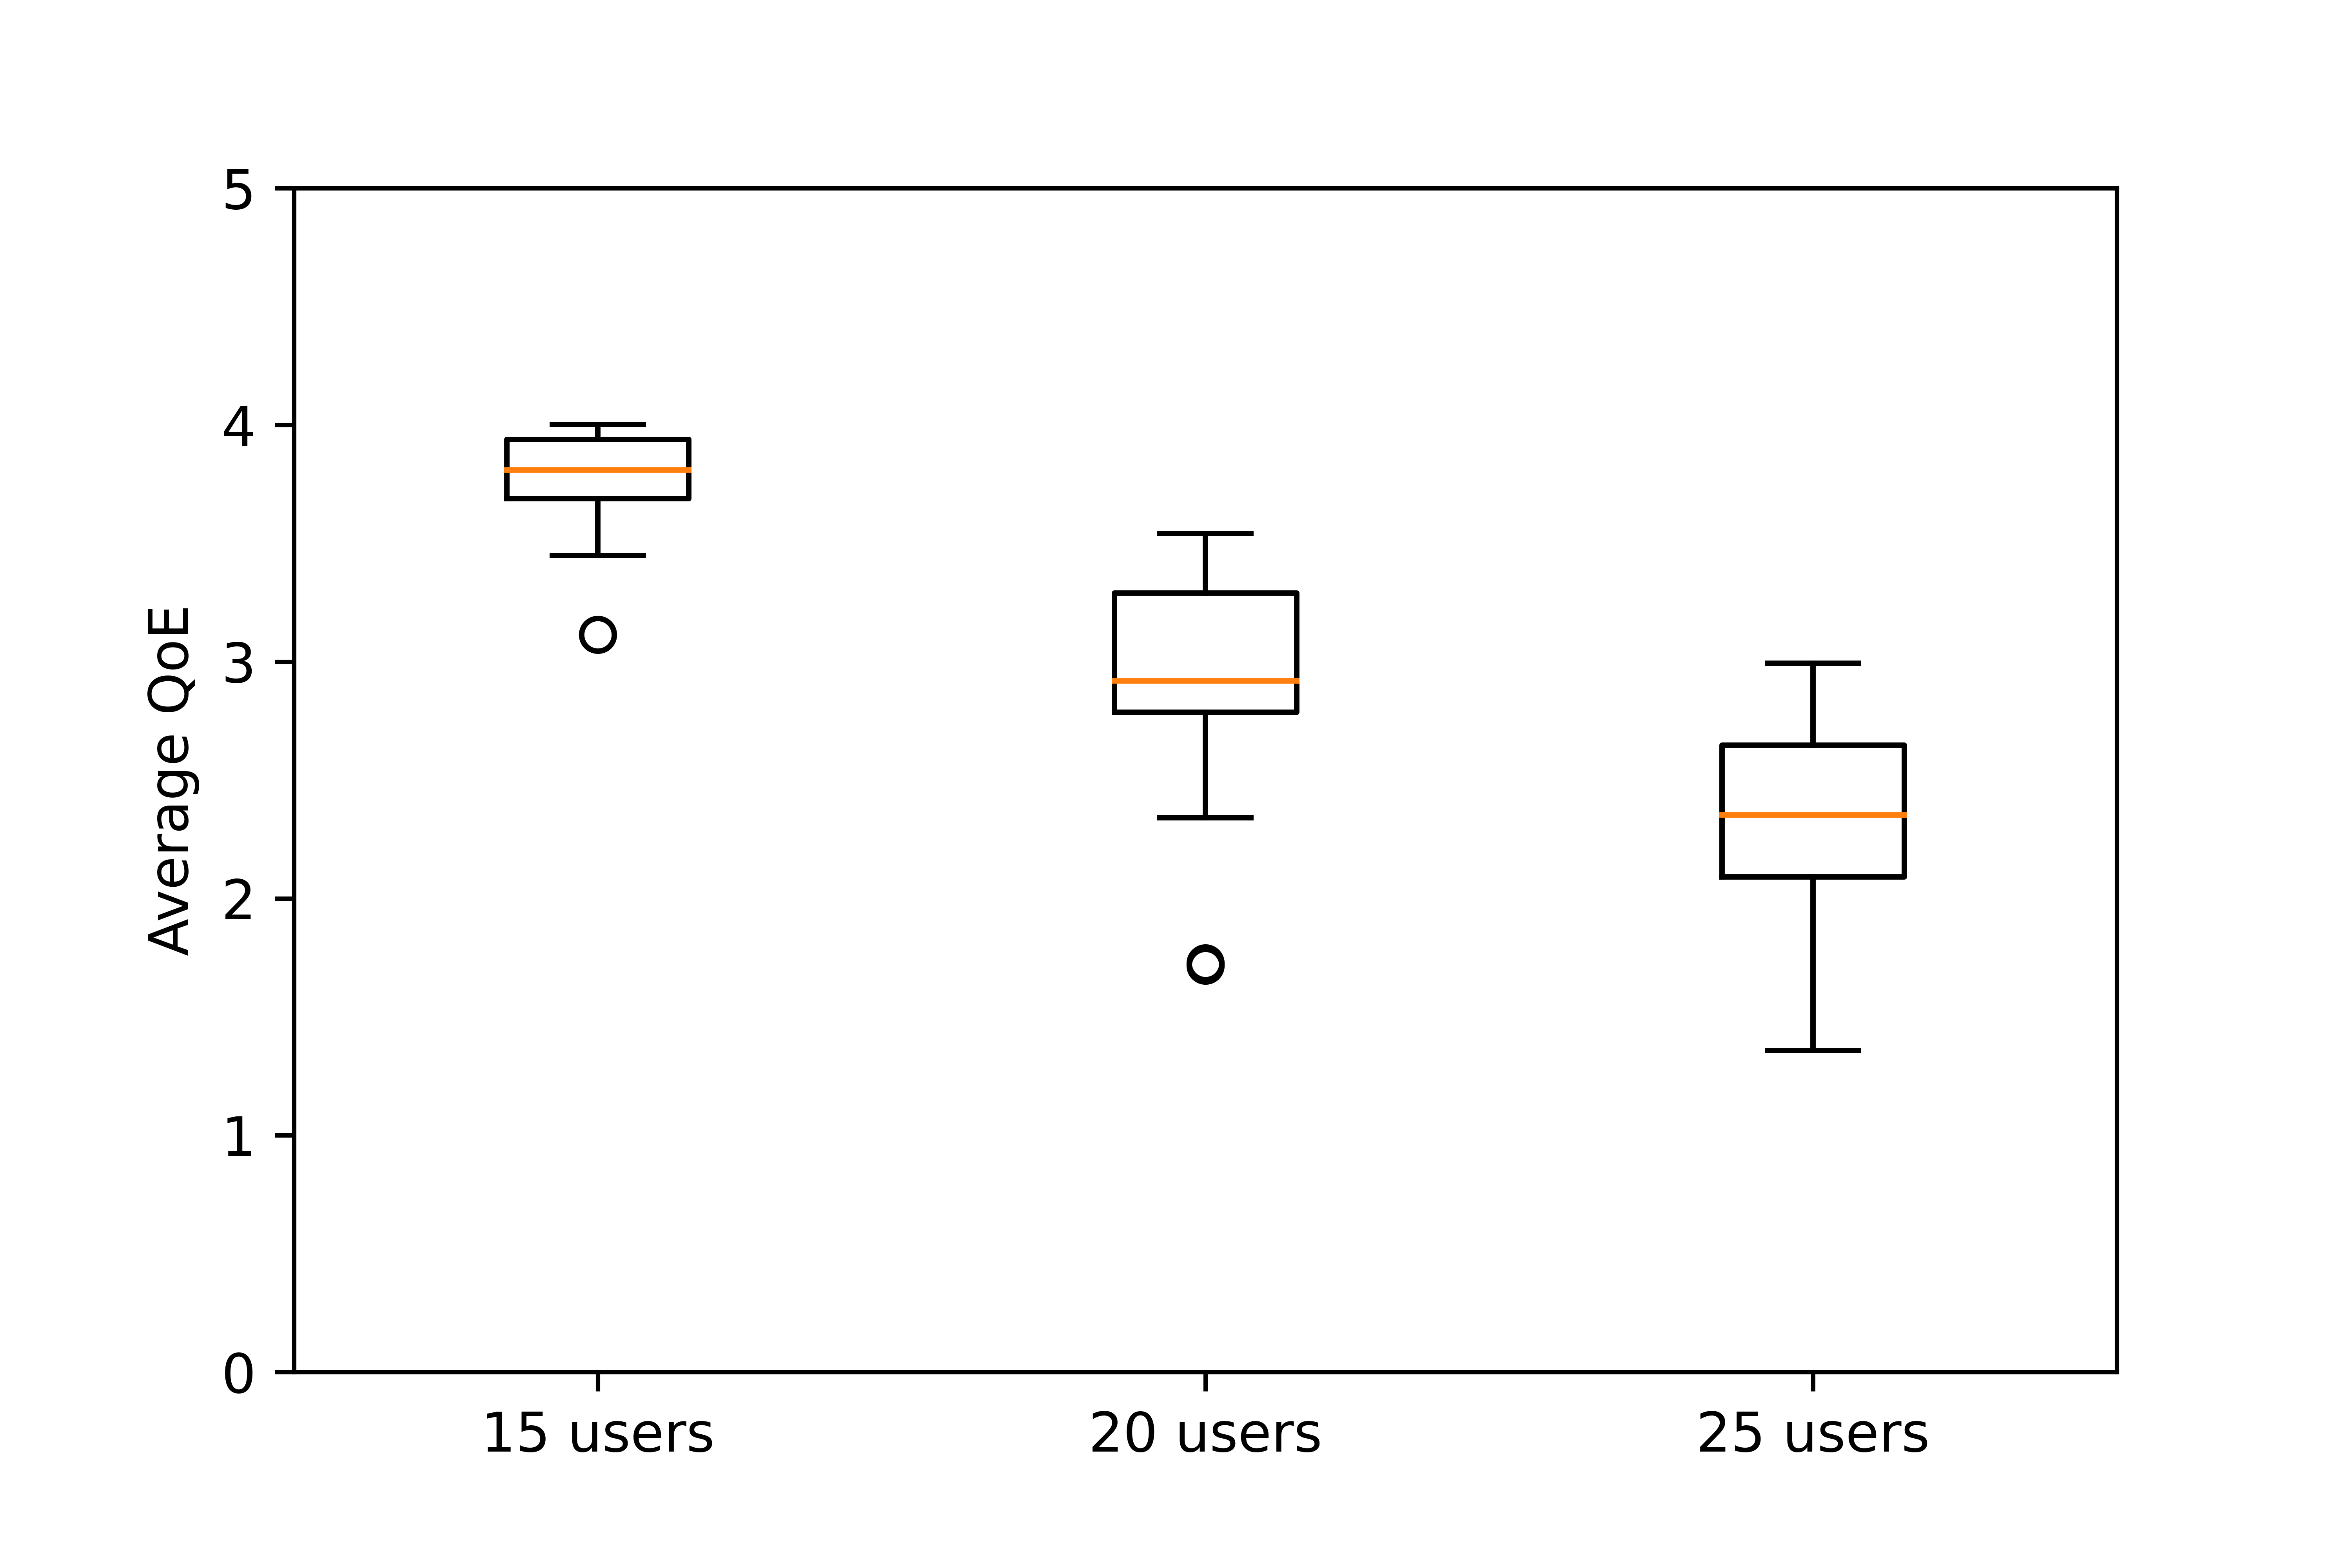
\includegraphics[width=0.45\linewidth]{images/QoEBoxplot.png}
%     \label{fig:co-comparison-boxplot}
%     }

%     \subfigure[]{
%     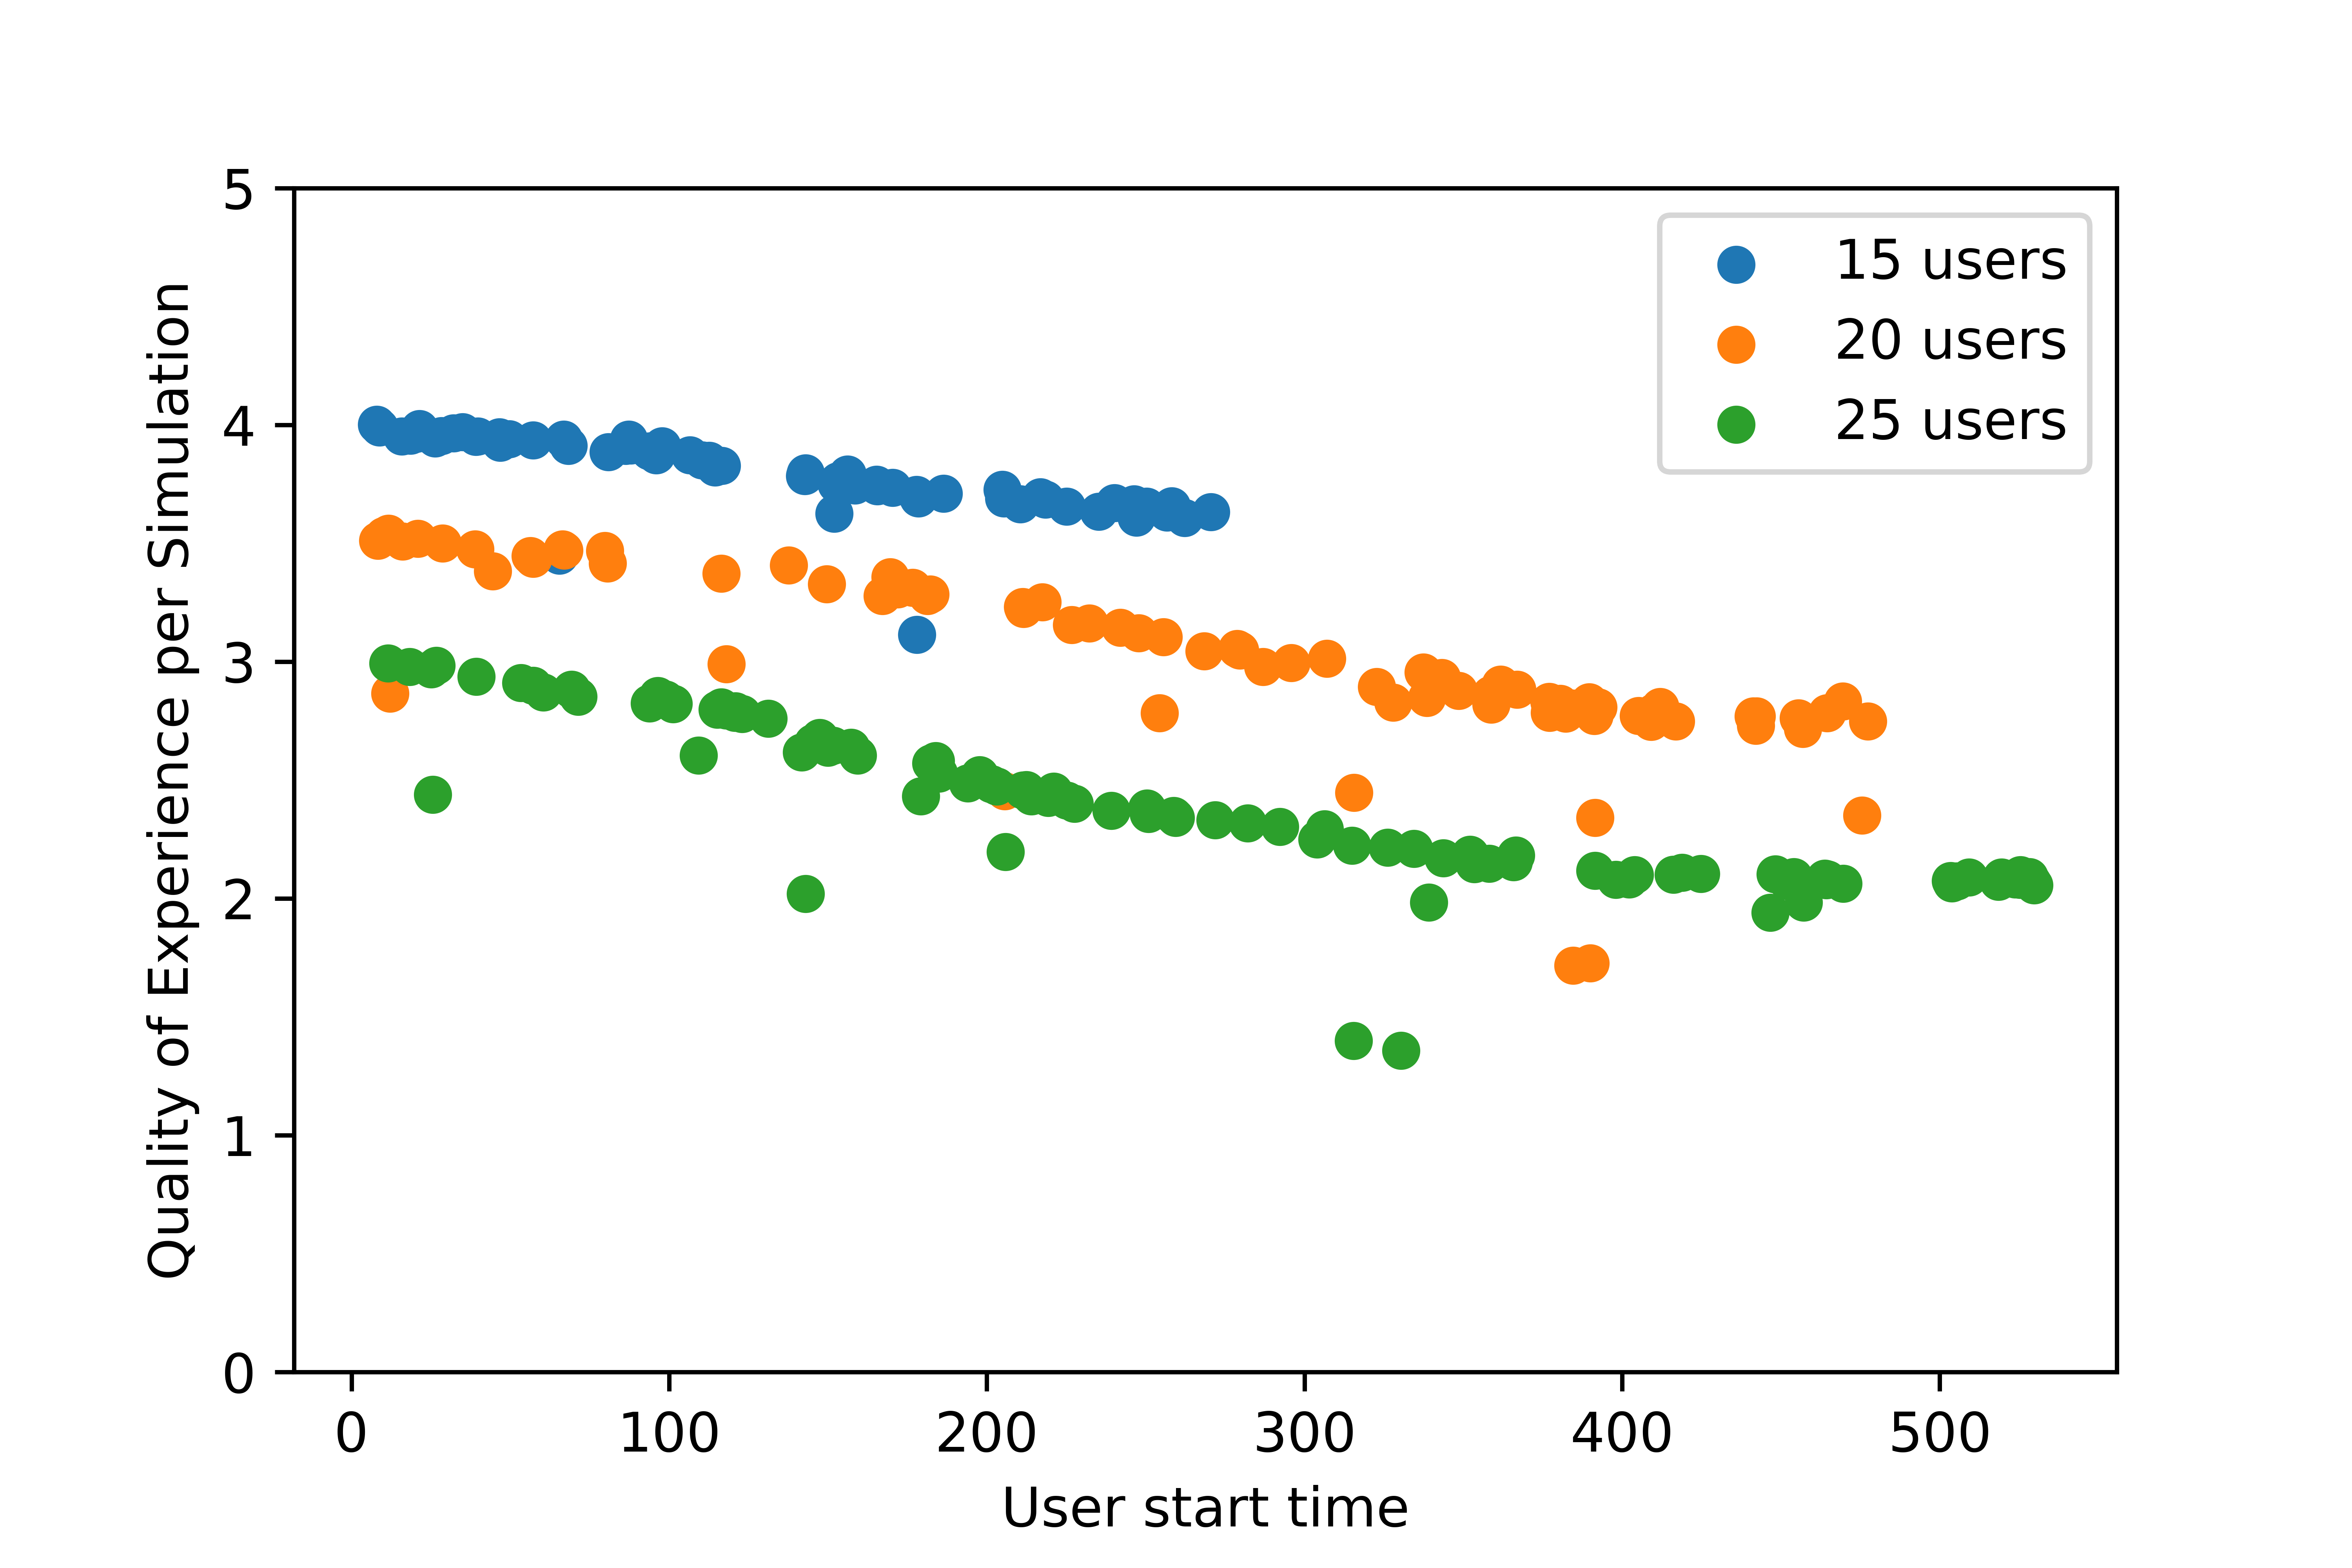
\includegraphics[width=0.45\linewidth]{images/QoECompare.png}
%     \label{fig:red-comparison-plot}
%     }
%     \subfigure[]{
%     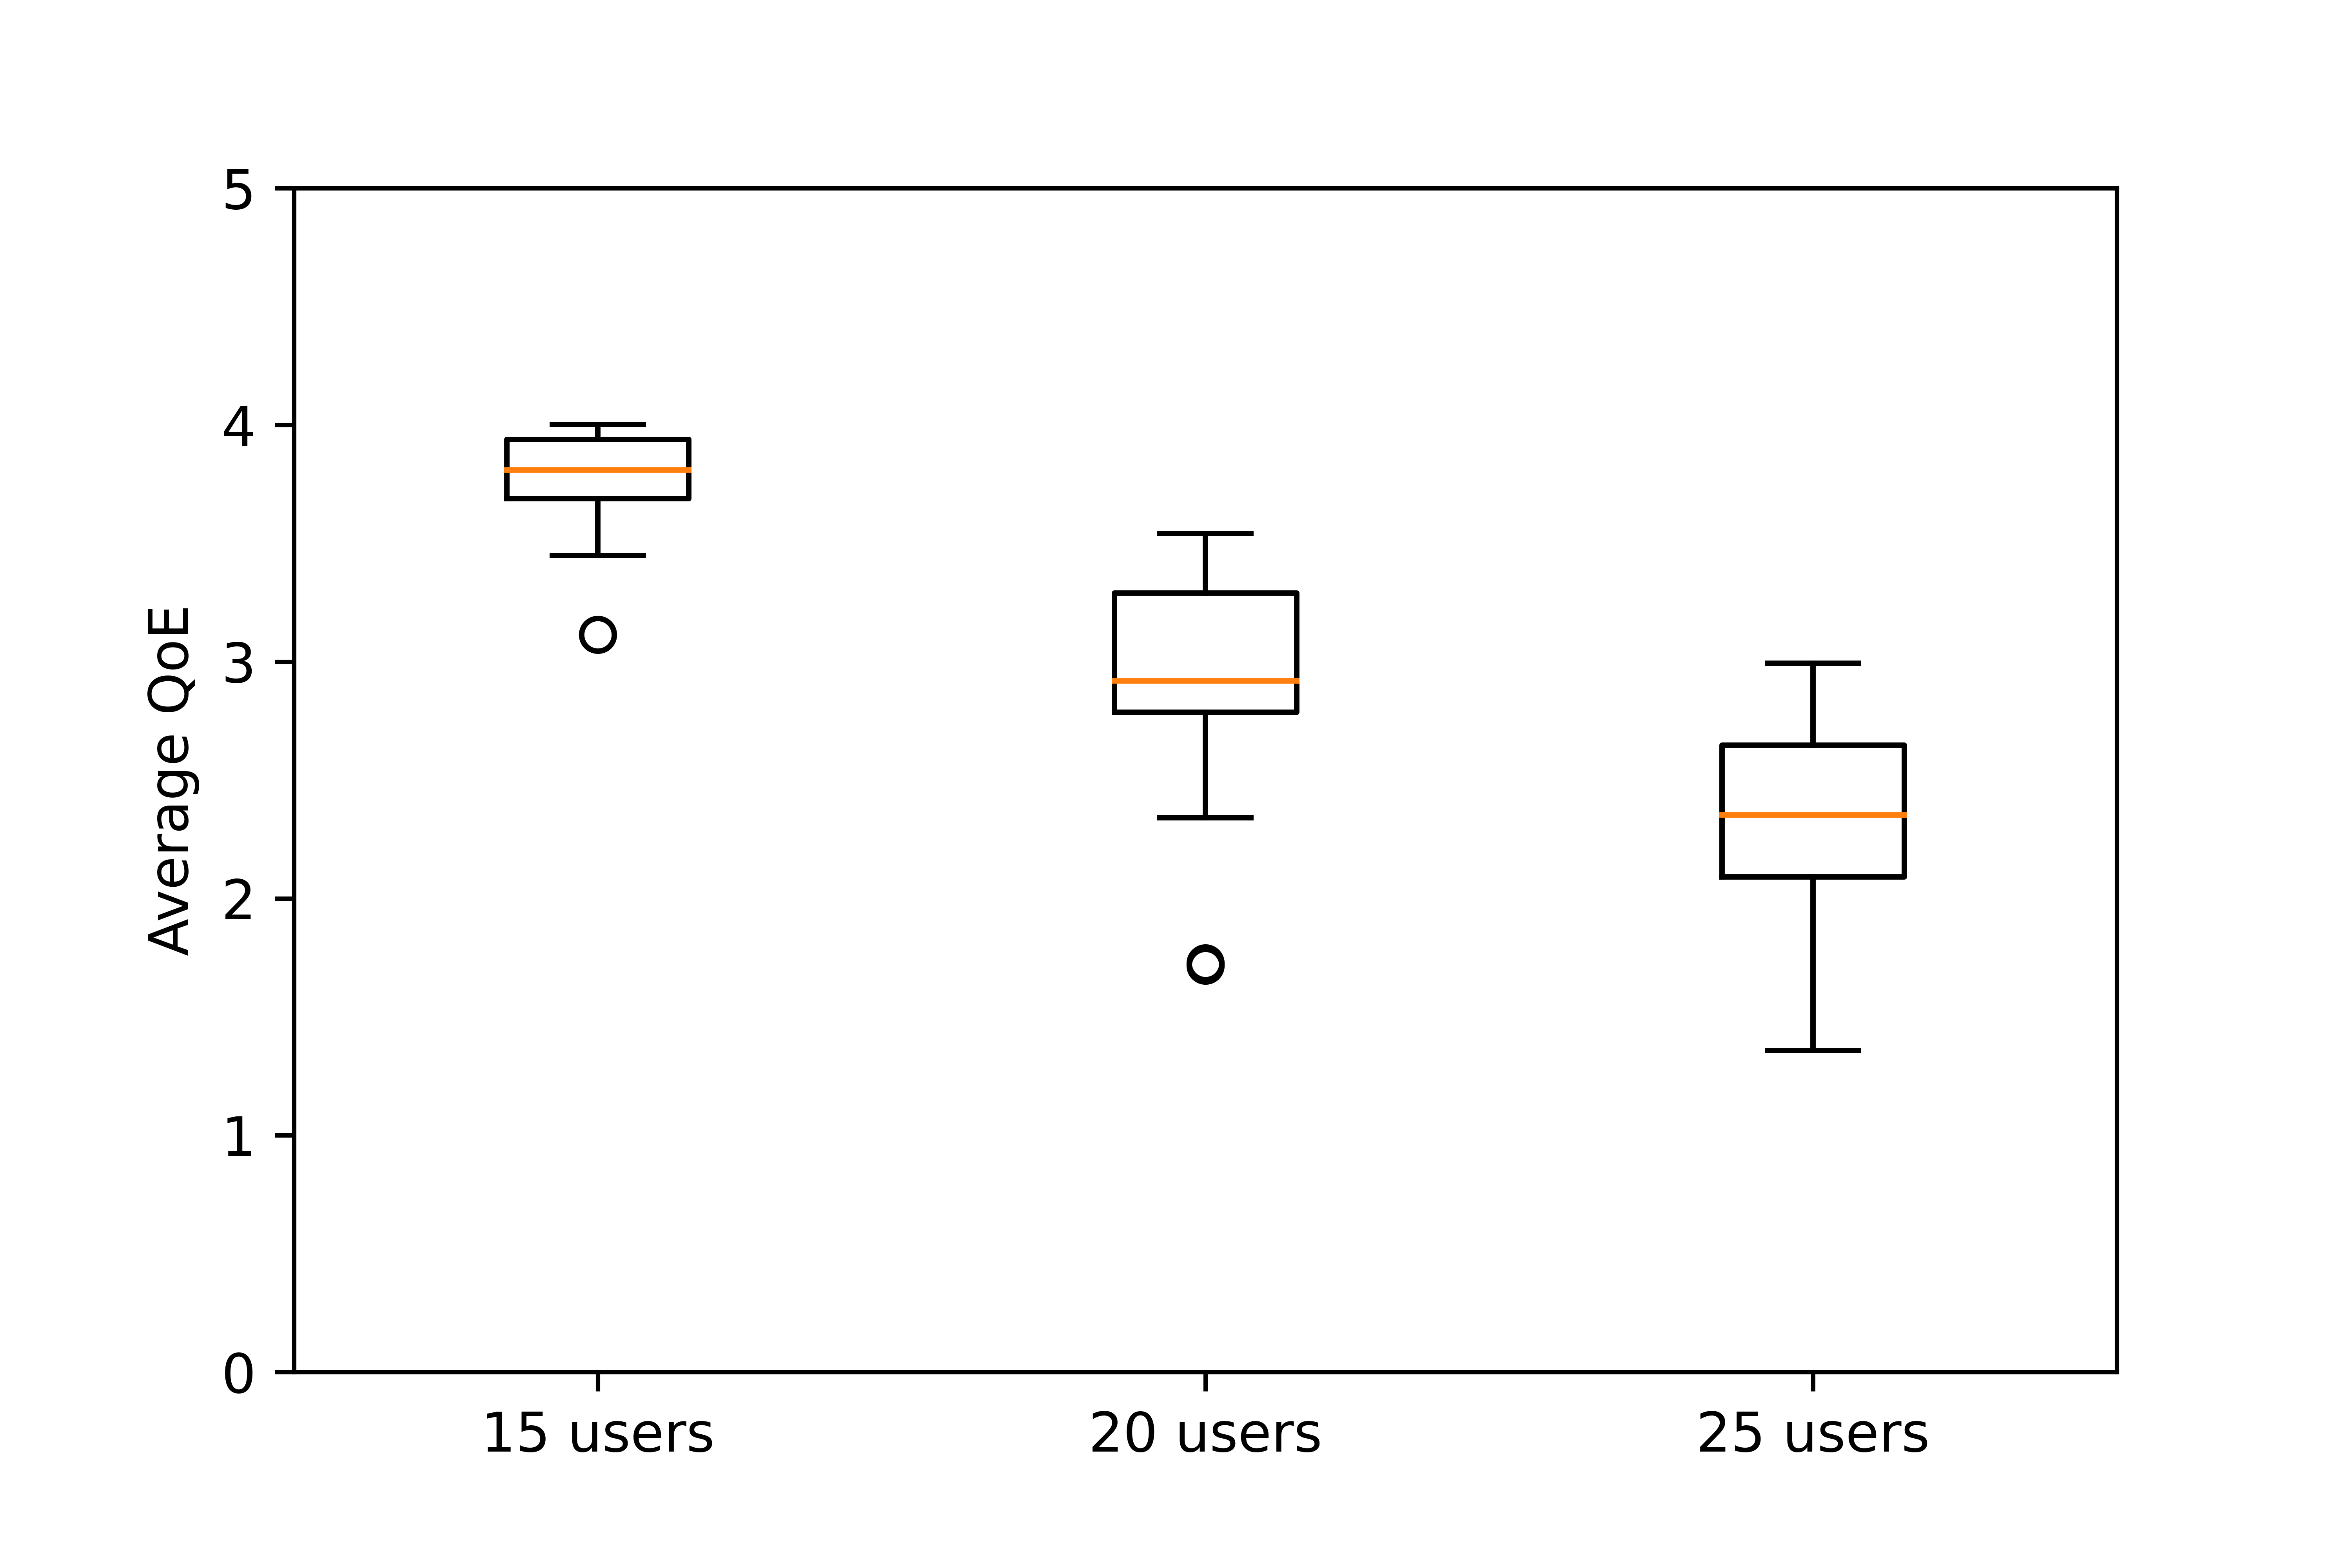
\includegraphics[width=0.45\linewidth]{images/QoEBoxplot.png}
%     \label{fig:red-comparison-boxplot}
%     }

%     \caption{Impact of system on the network performance. Distance \textit{d} between sensor node and antennas of 8m in a semi-NLOS scenario.}
%     \label{fig:comparison-rof-2}
% \end{figure*}

\begin{figure*}
    \centering
    \subfigure[]{
    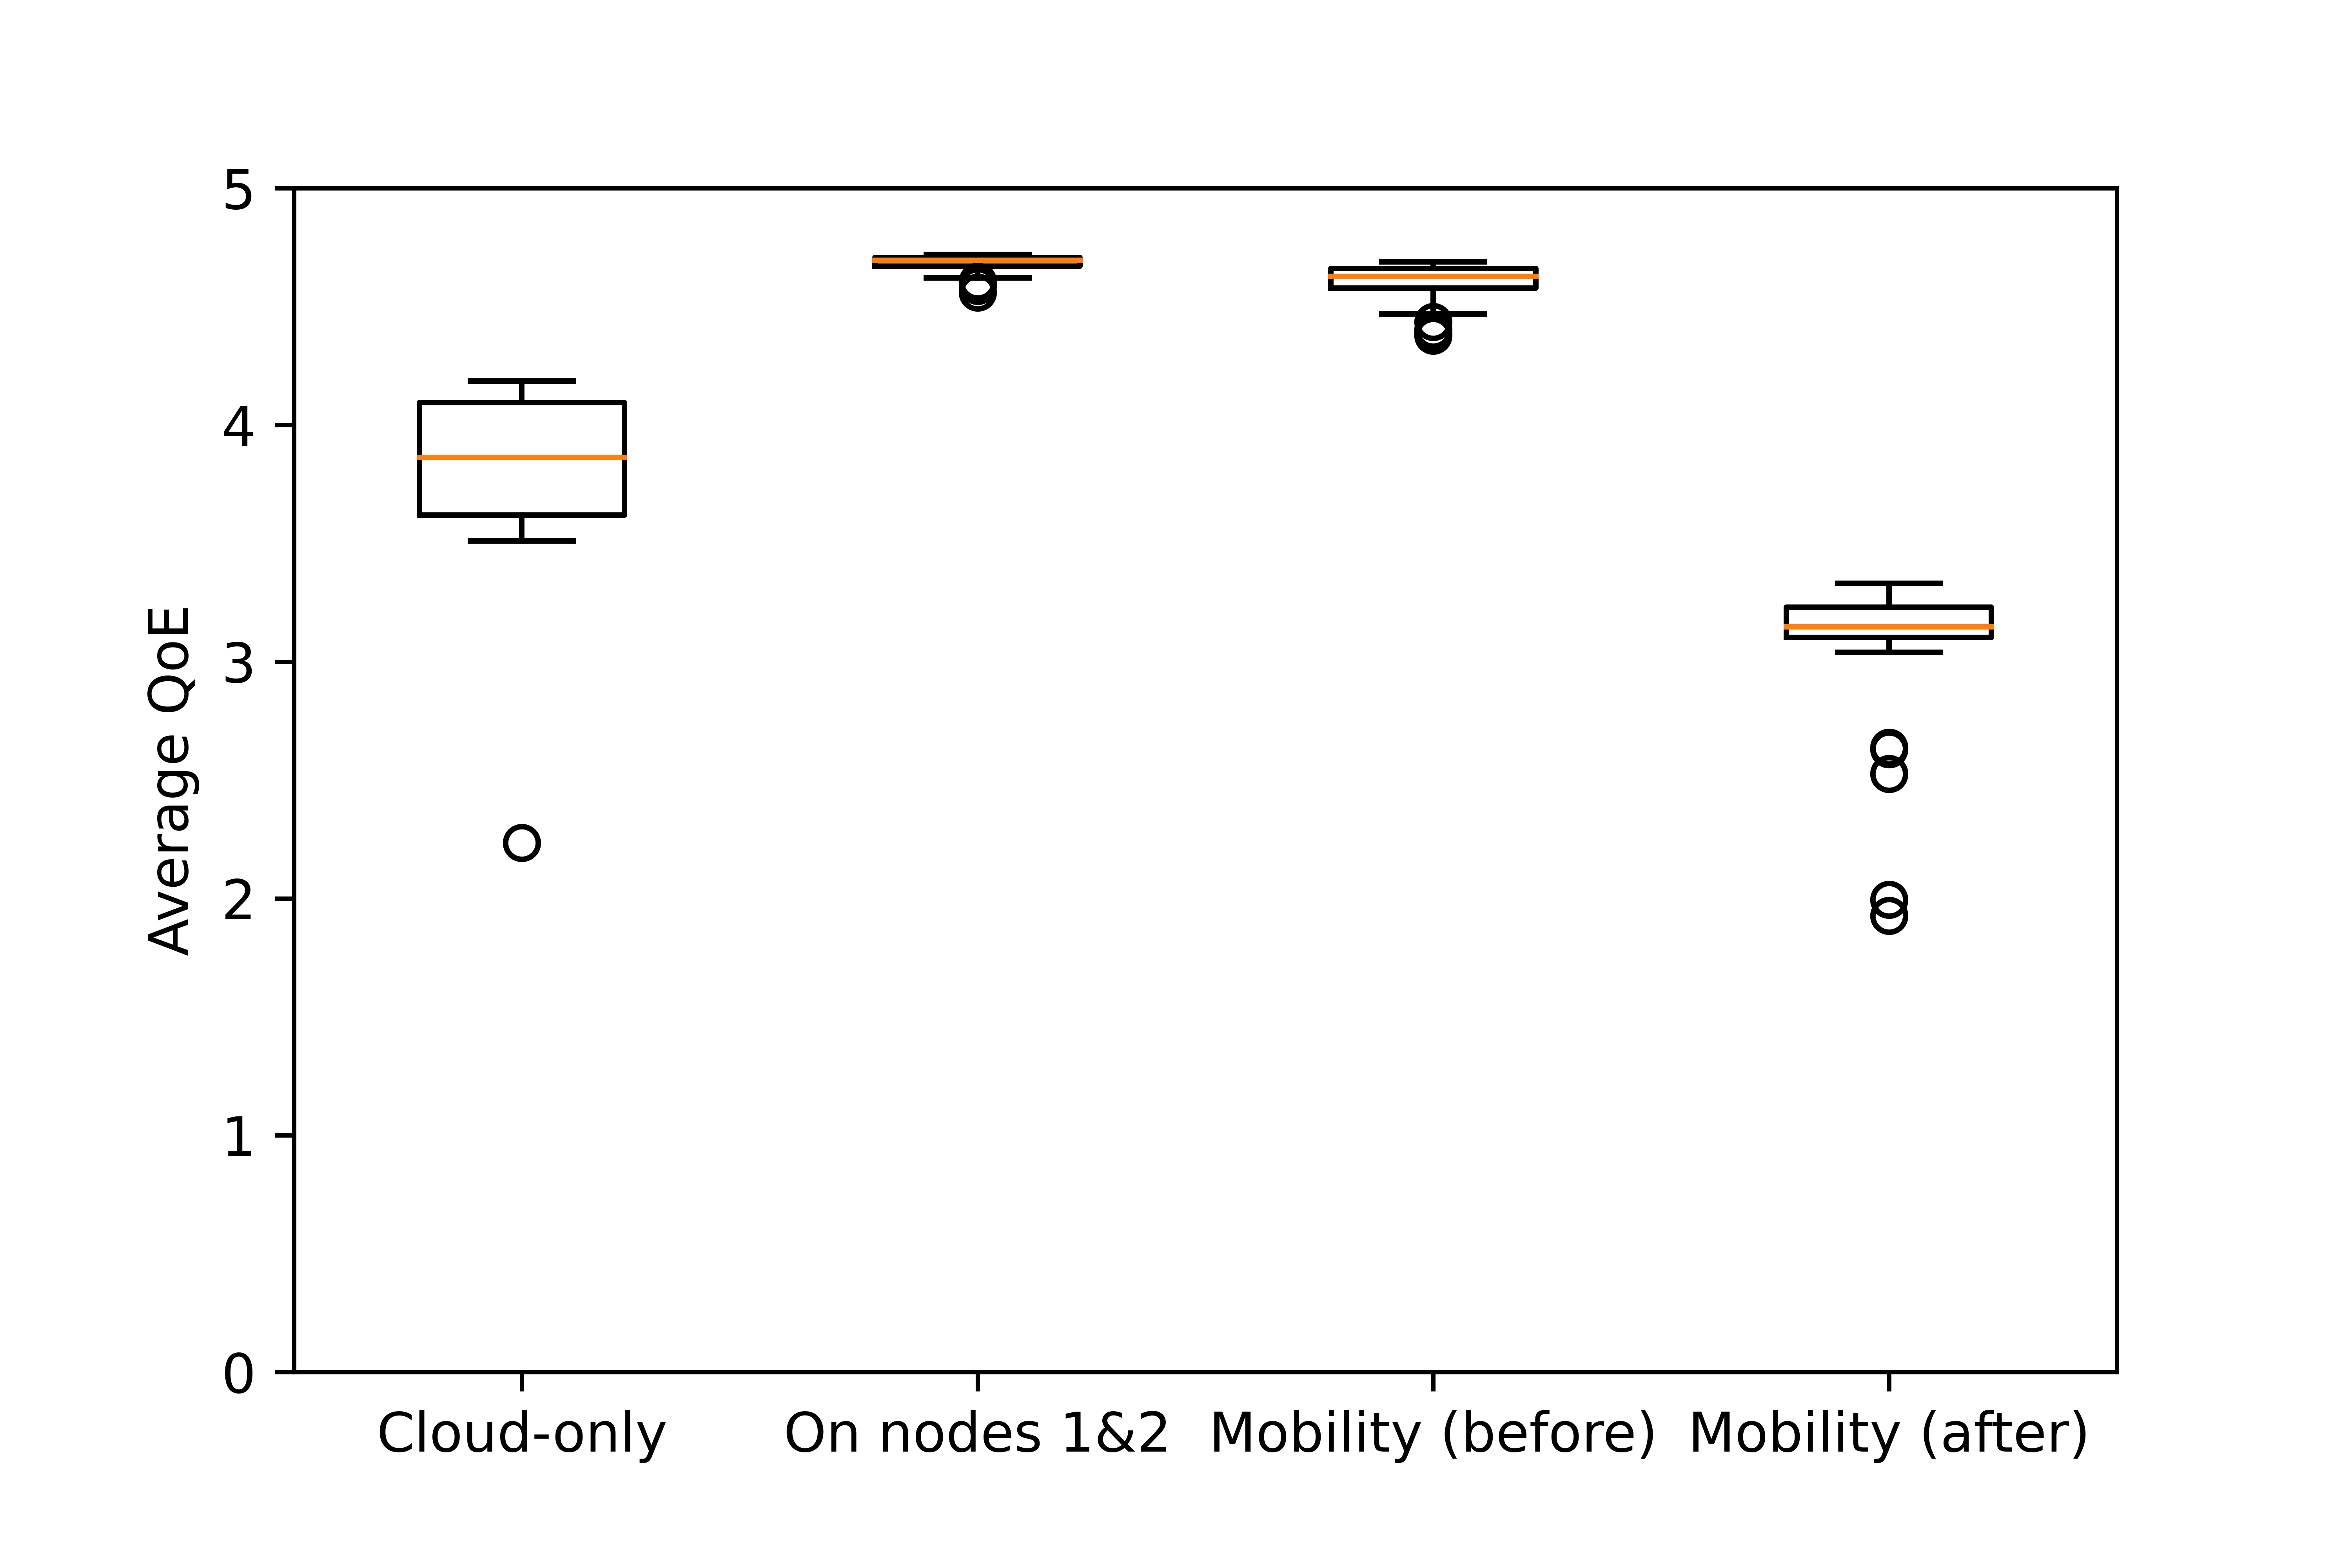
\includegraphics[width=0.31\linewidth]{images/QoEBoxplot-15u.png}
    \label{fig:red-comparison-plot}
    }
    \subfigure[]{
    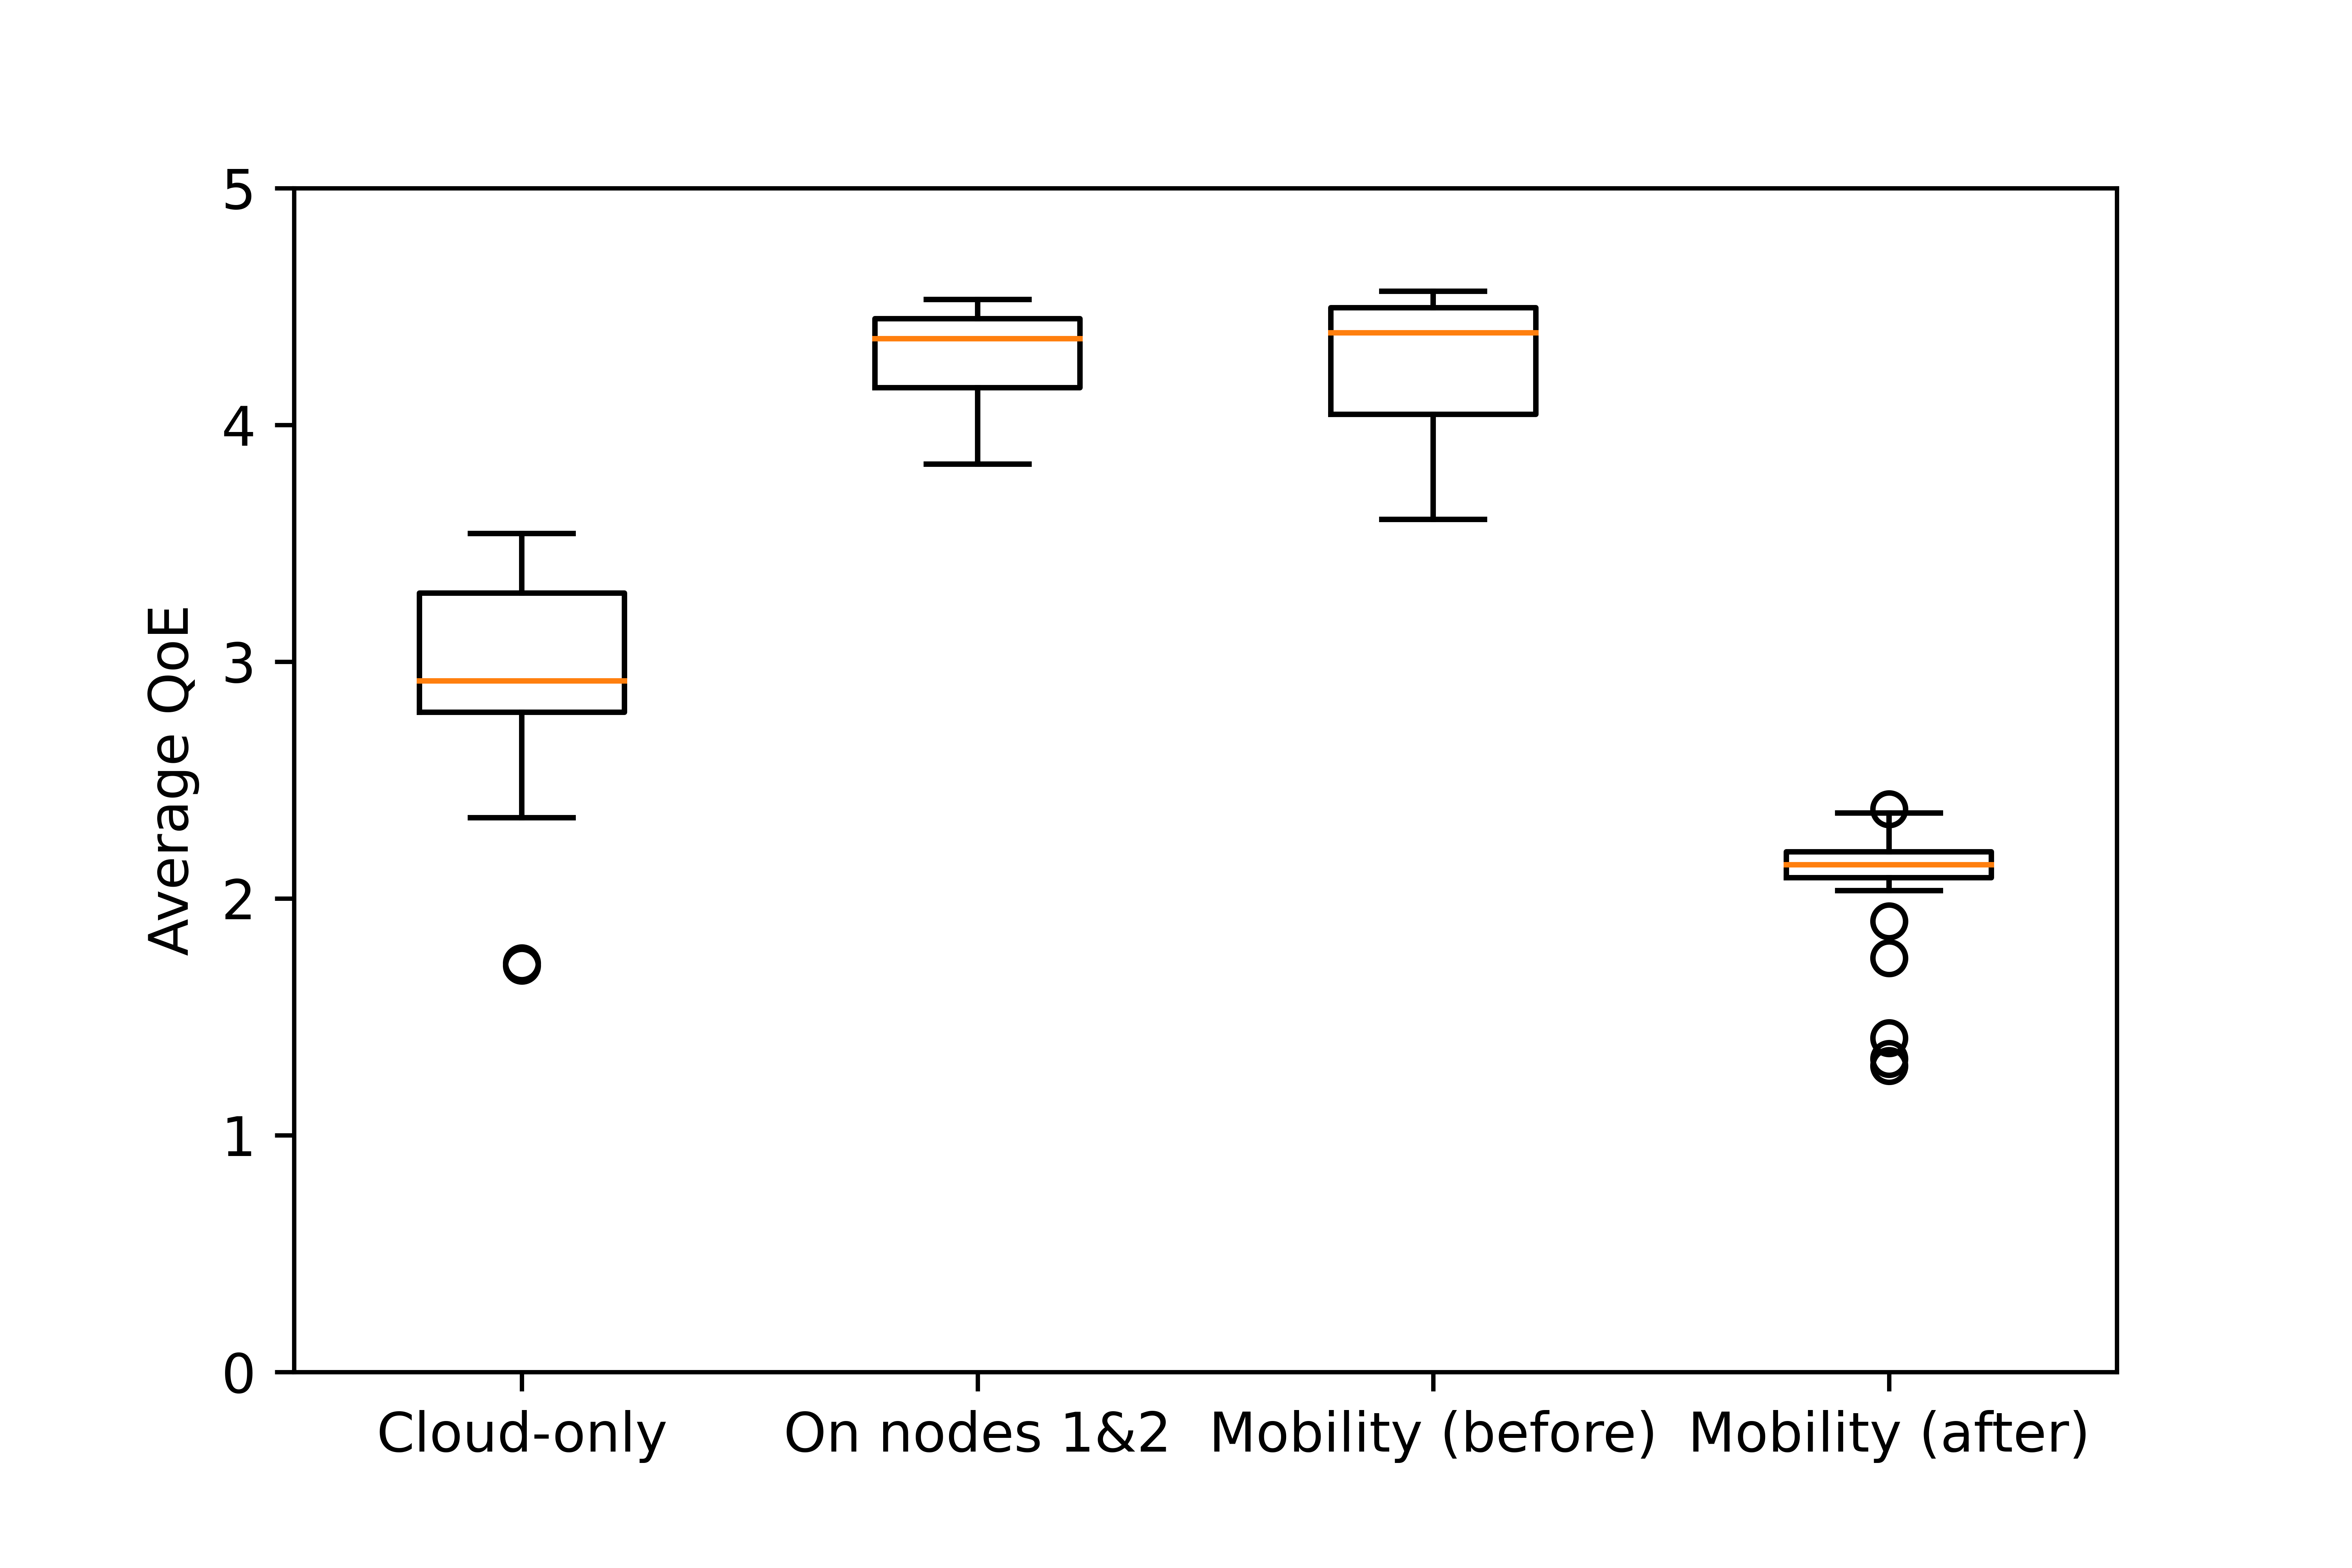
\includegraphics[width=0.31\linewidth]{images/QoEBoxplot-20u.png}
    \label{fig:co-comparison-boxplot}
    }
    \subfigure[]{
    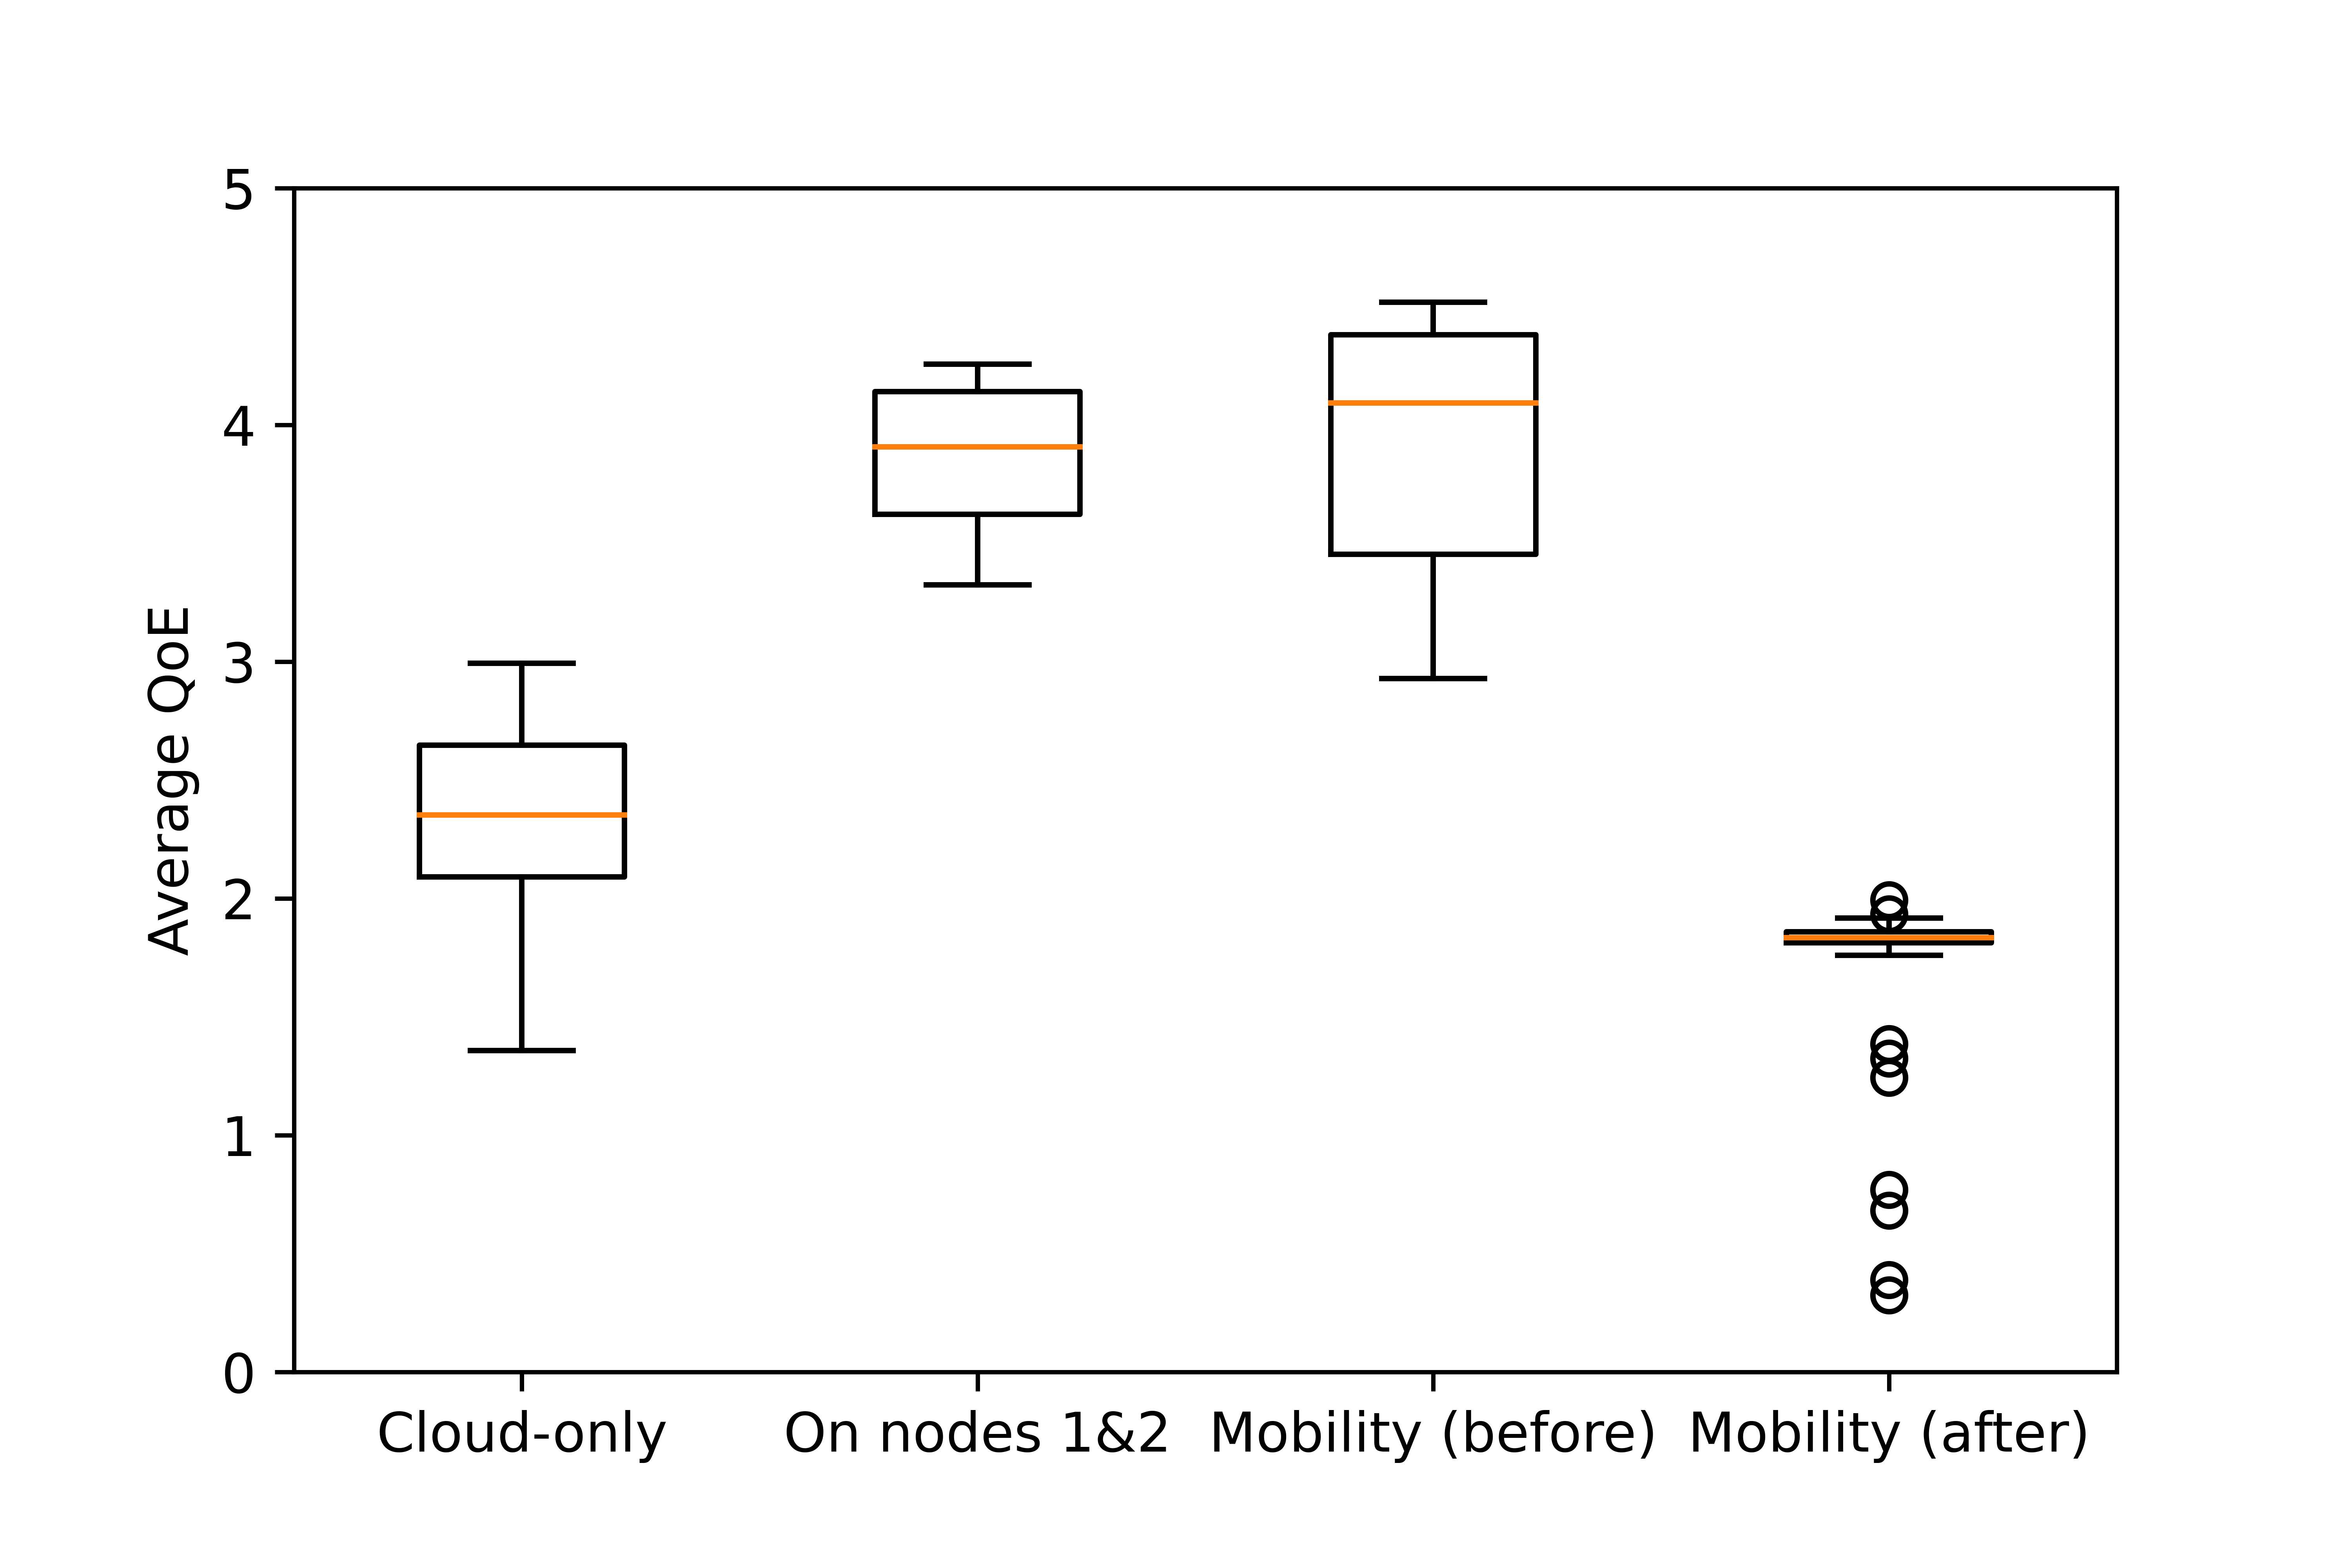
\includegraphics[width=0.31\linewidth]{images/QoEBoxplot-25u.png}
    \label{fig:red-comparison-plot}
    }
    
    \caption{Average QoE results for scenarios with 15, 20 and 25 users per AP.}
    \label{fig:comparison-rof-2}
\end{figure*}


\begin{figure*}
    \centering
    \subfigure[]{
    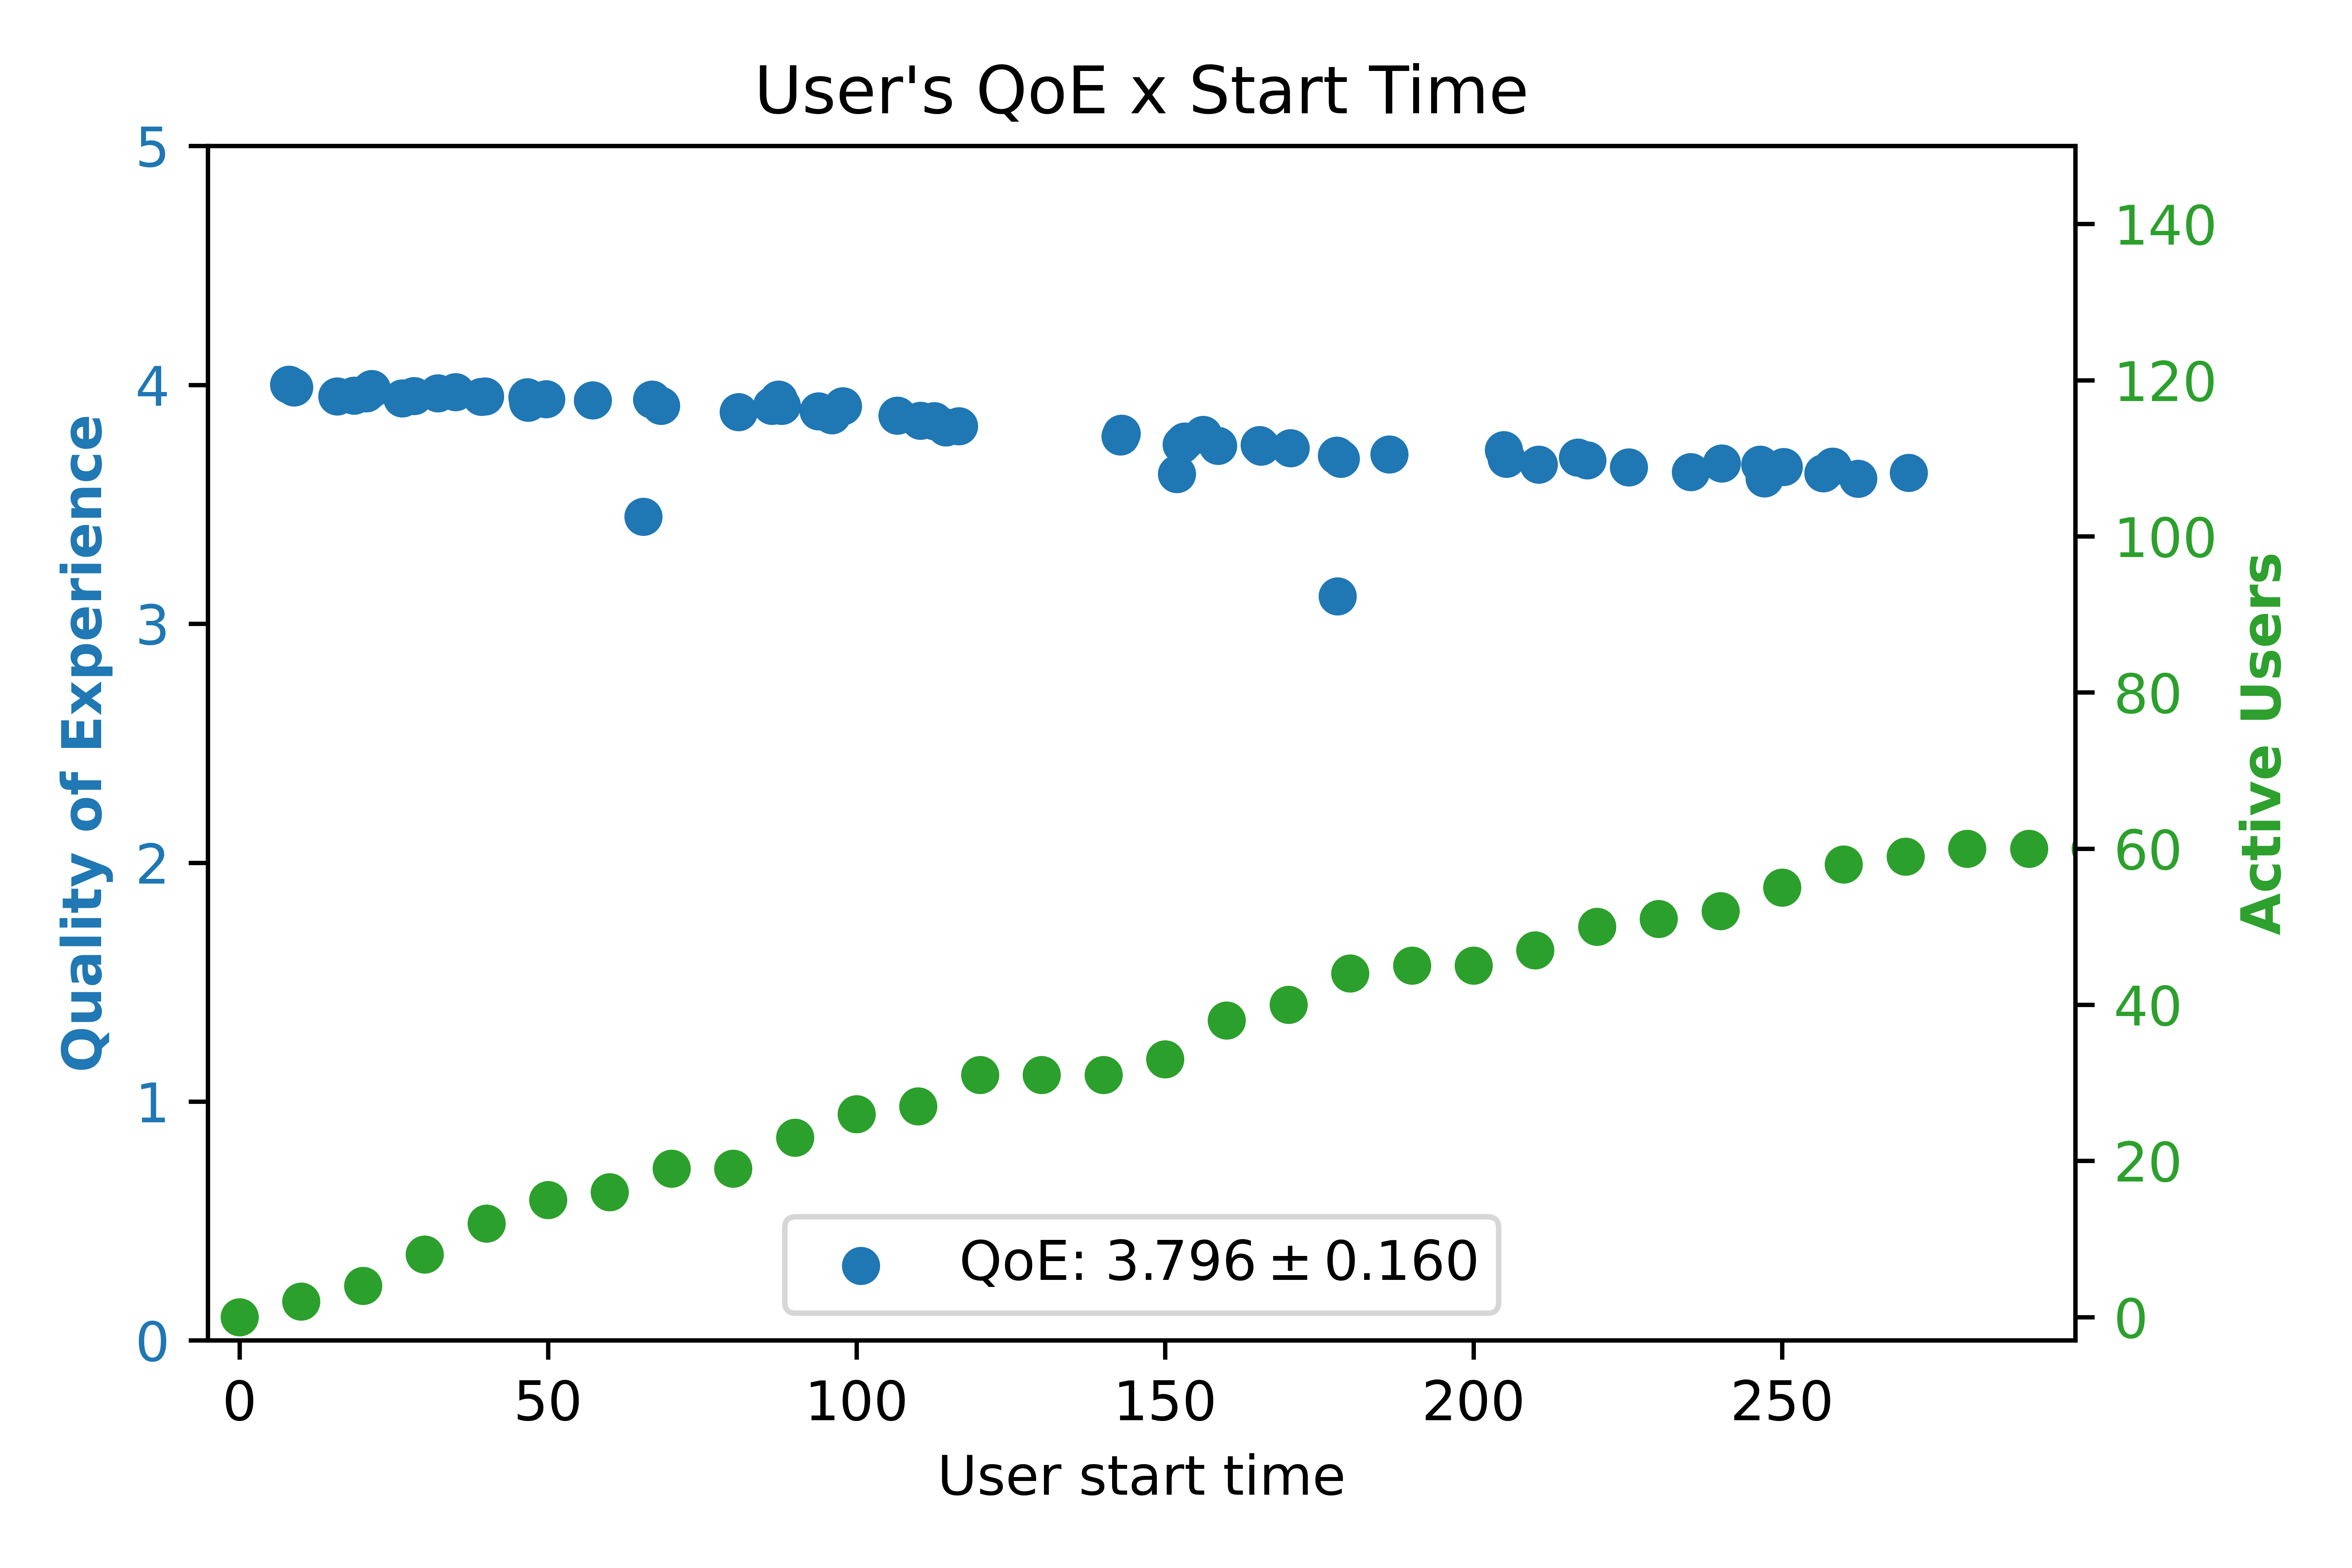
\includegraphics[width=0.31\linewidth]{images/cloud_QoExStartTime15.png}
    \label{fig:rssi-comparison-2}
    }
    \subfigure[]{
    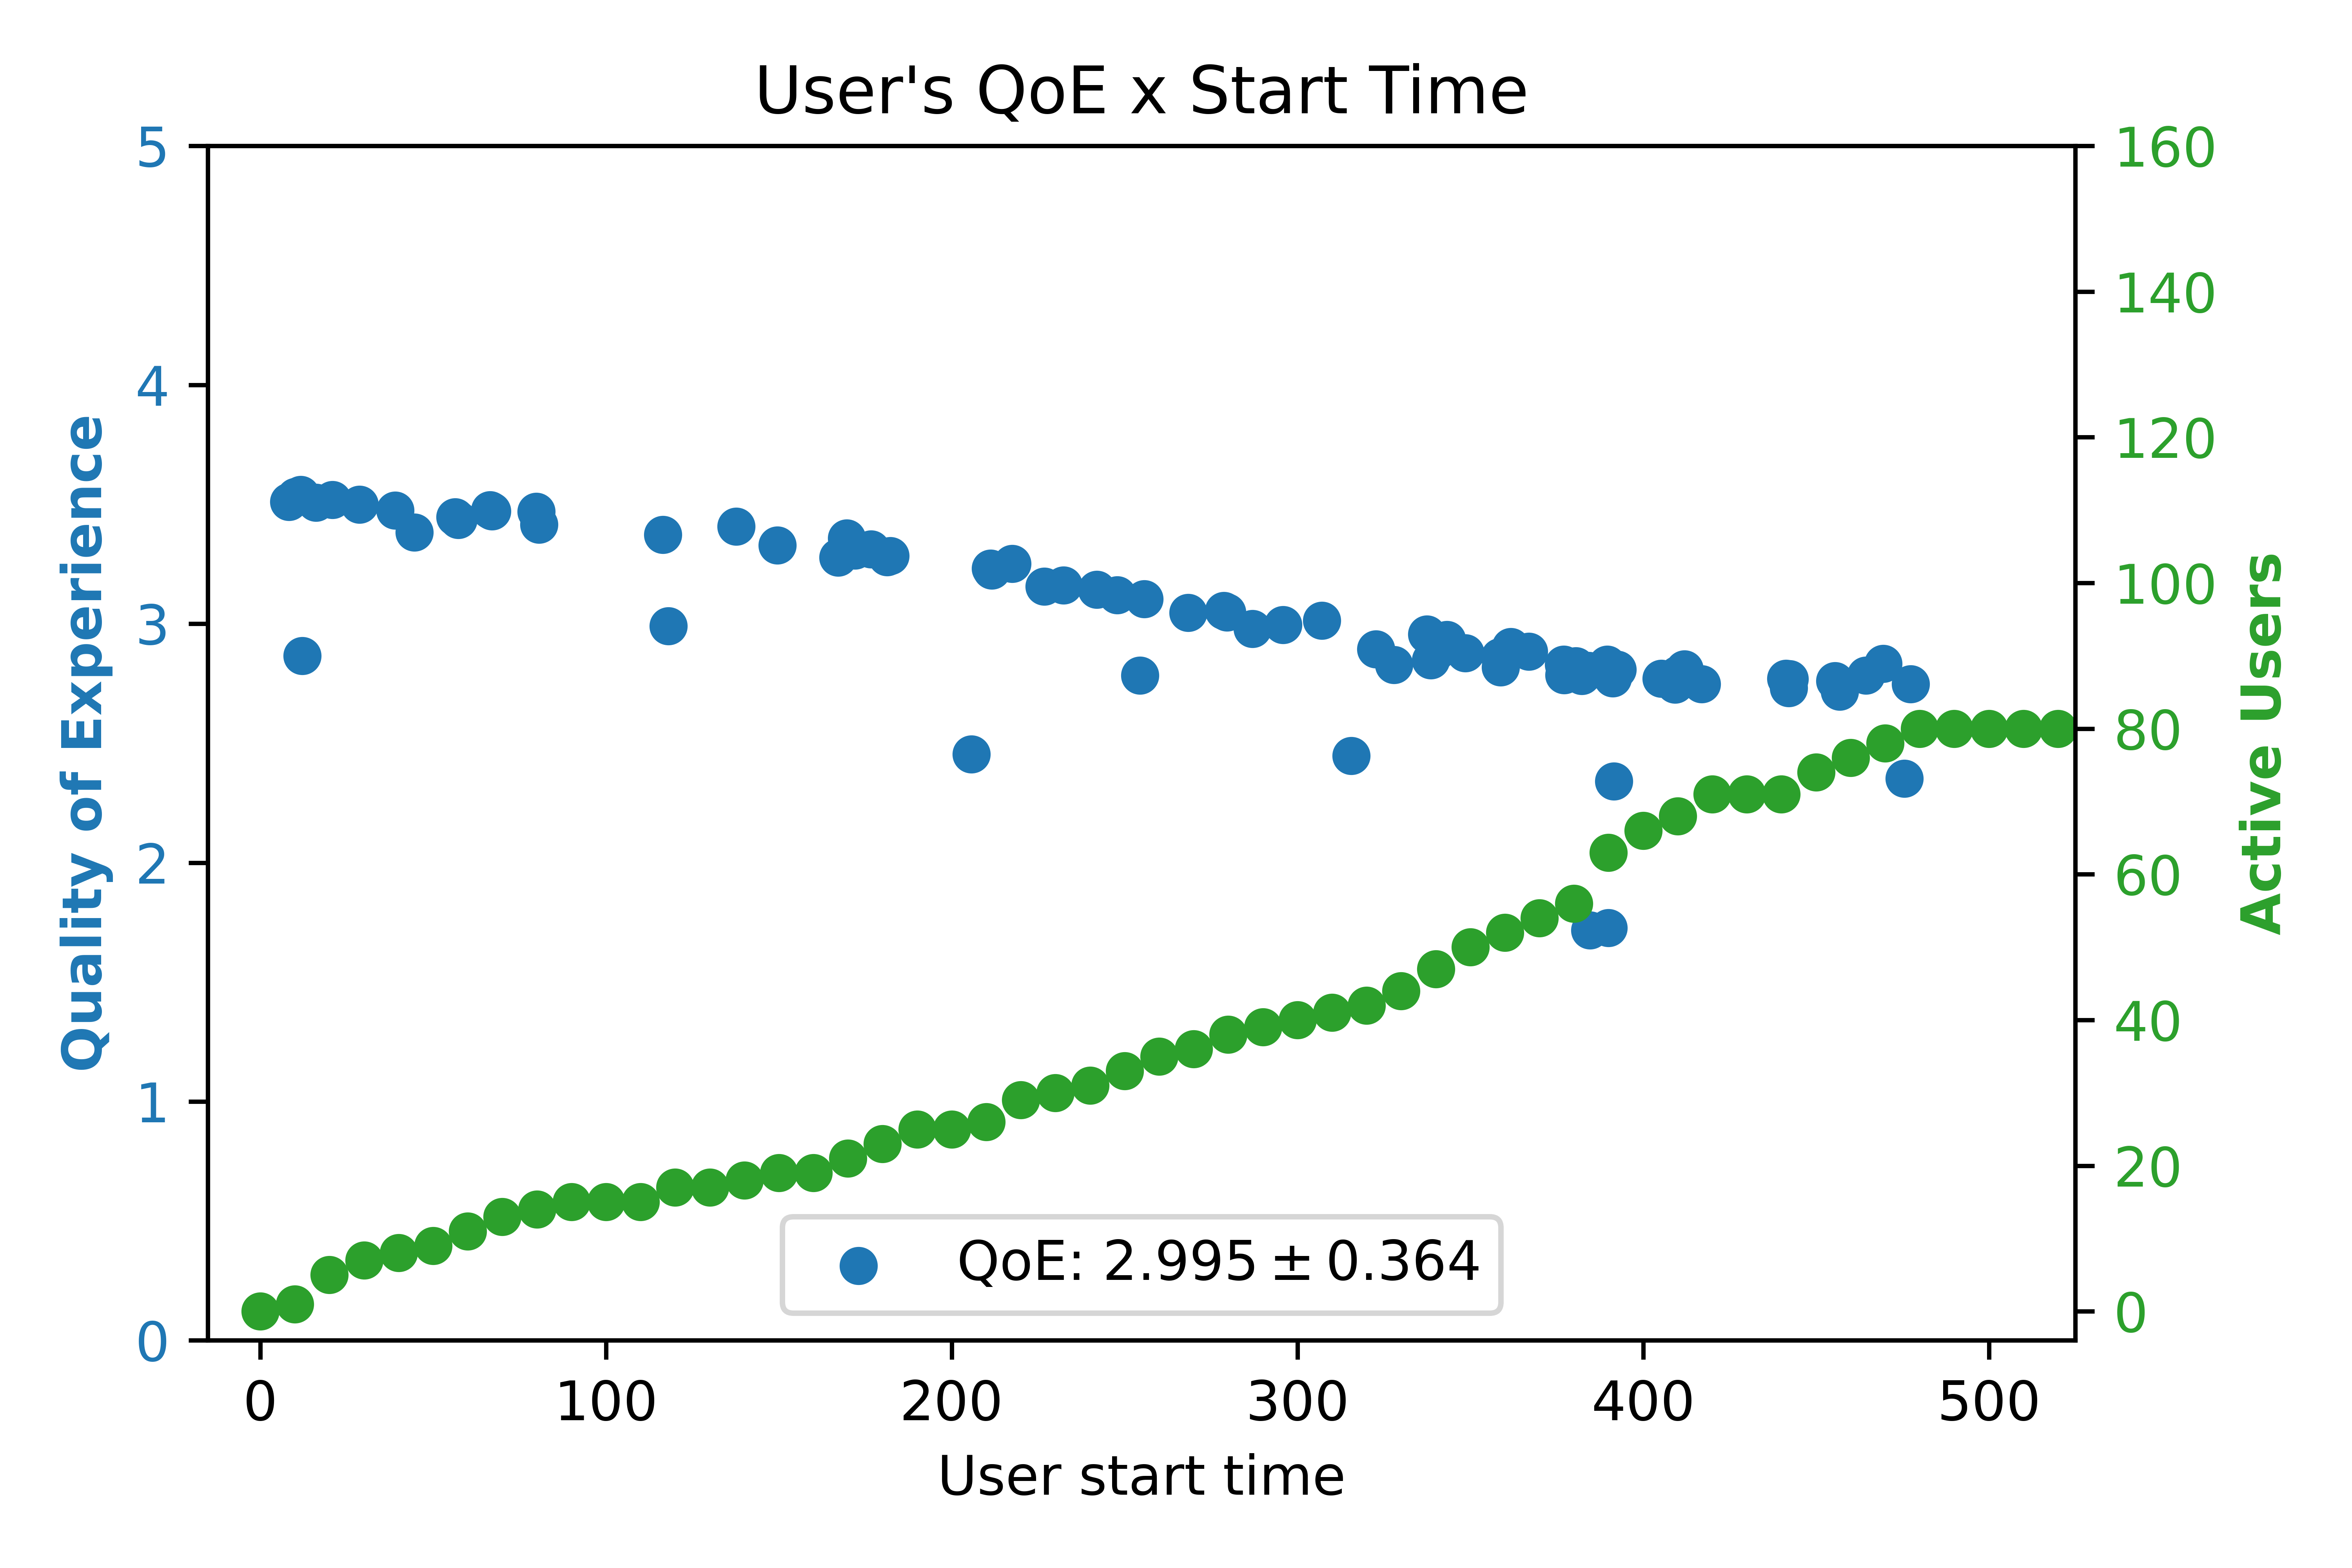
\includegraphics[width=0.31\linewidth]{images/cloud_QoExStartTime20.png}
    \label{fig:plr-comparison-2}
    }
    \subfigure[]{
    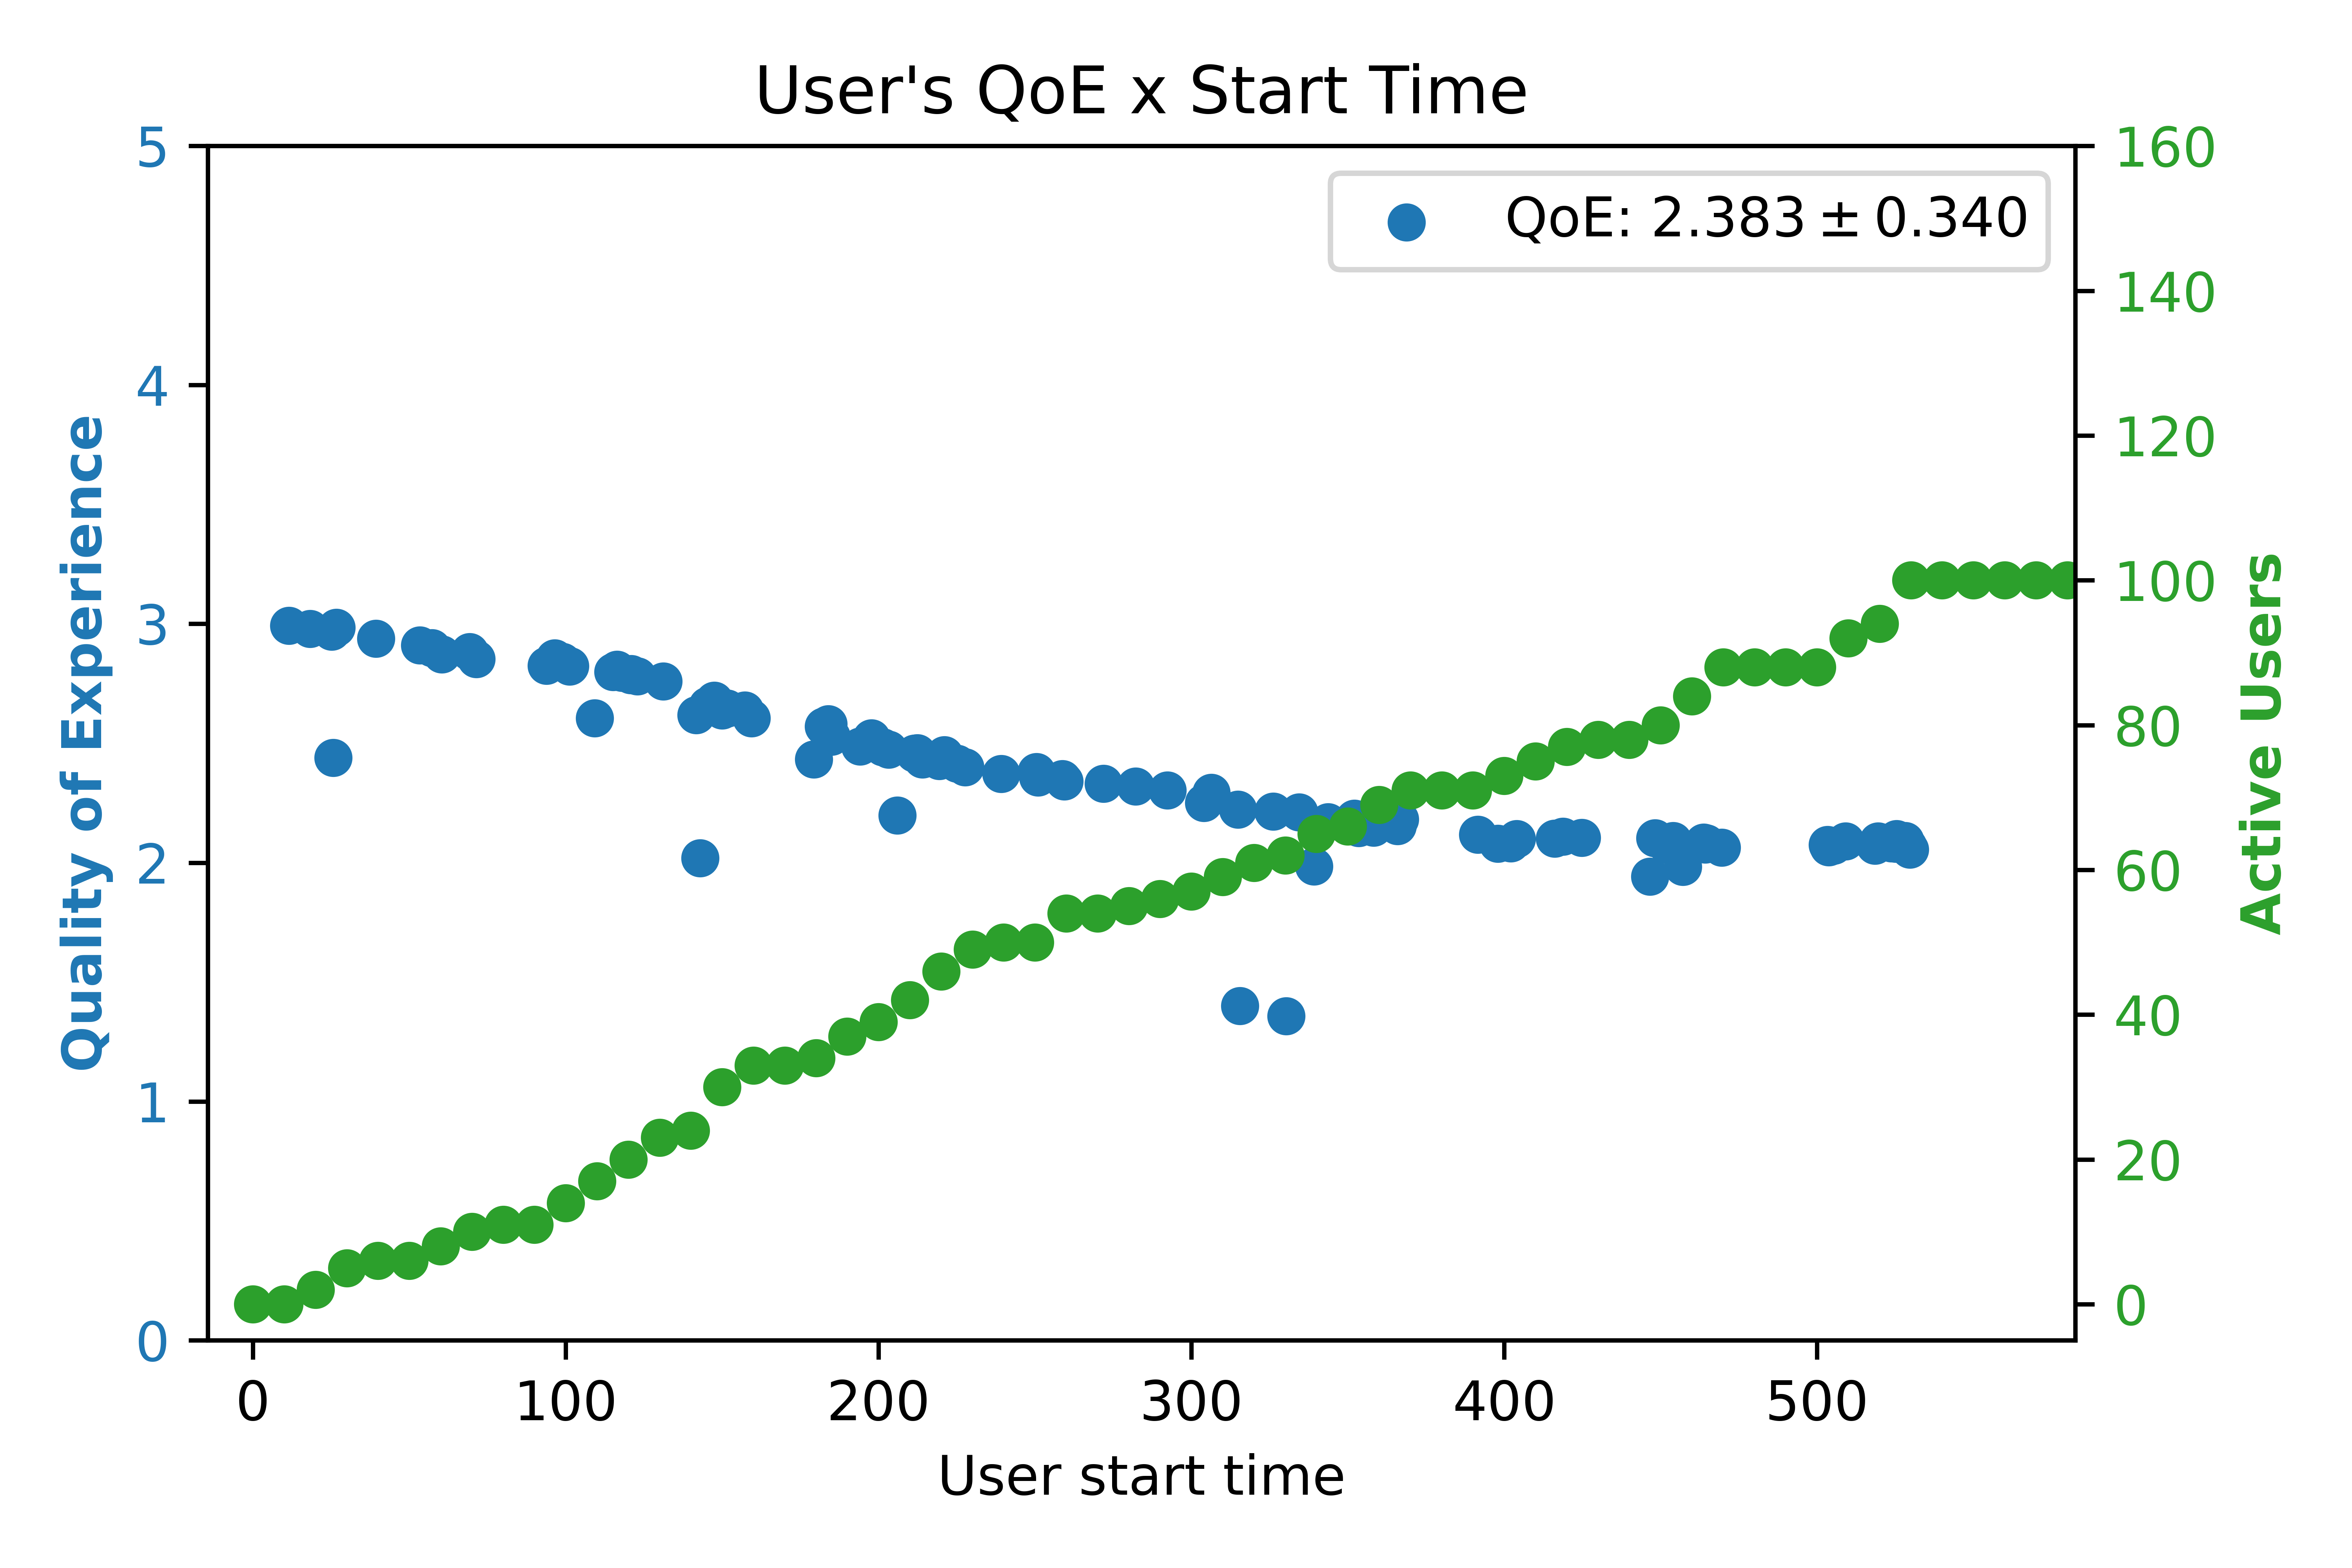
\includegraphics[width=0.31\linewidth]{images/cloud_QoExStartTime25.png}
    \label{fig:plr-comparison-2}
    }
    
    \subfigure[]{
    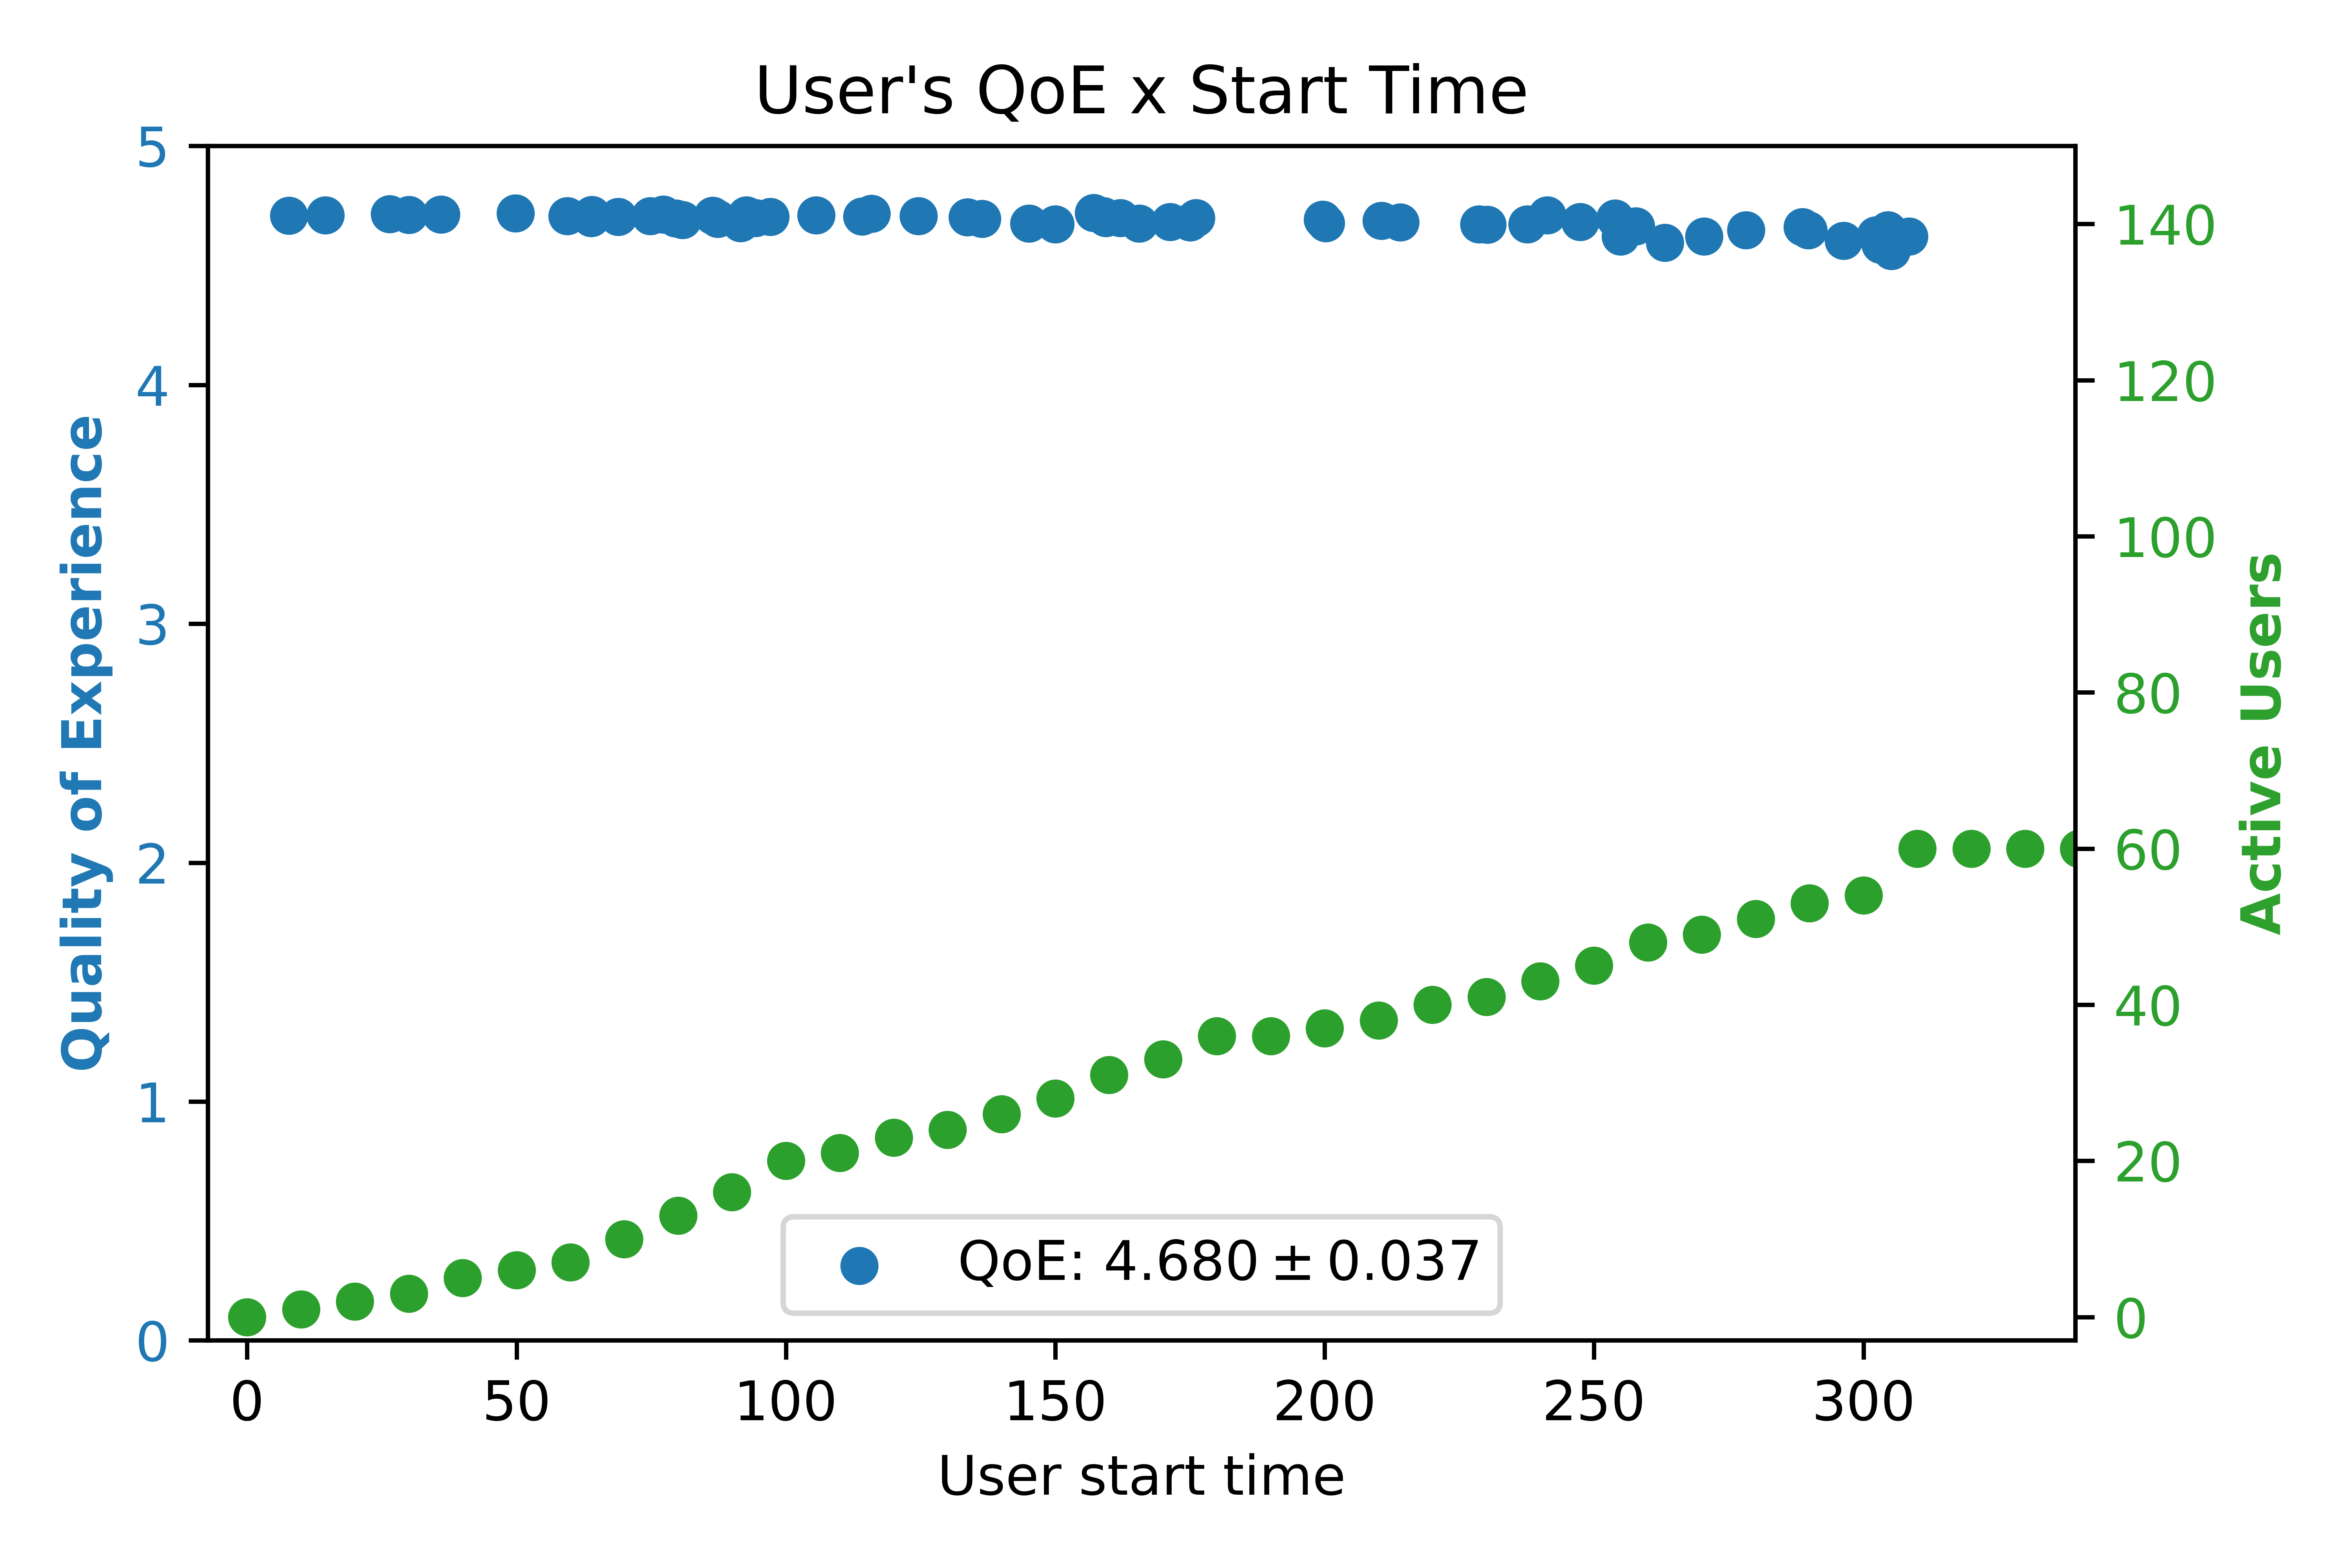
\includegraphics[width=0.31\linewidth]{images/Redicrect_QoExStartTime15.png}
    \label{fig:rssi-comparison-2}
    }
    \subfigure[]{
    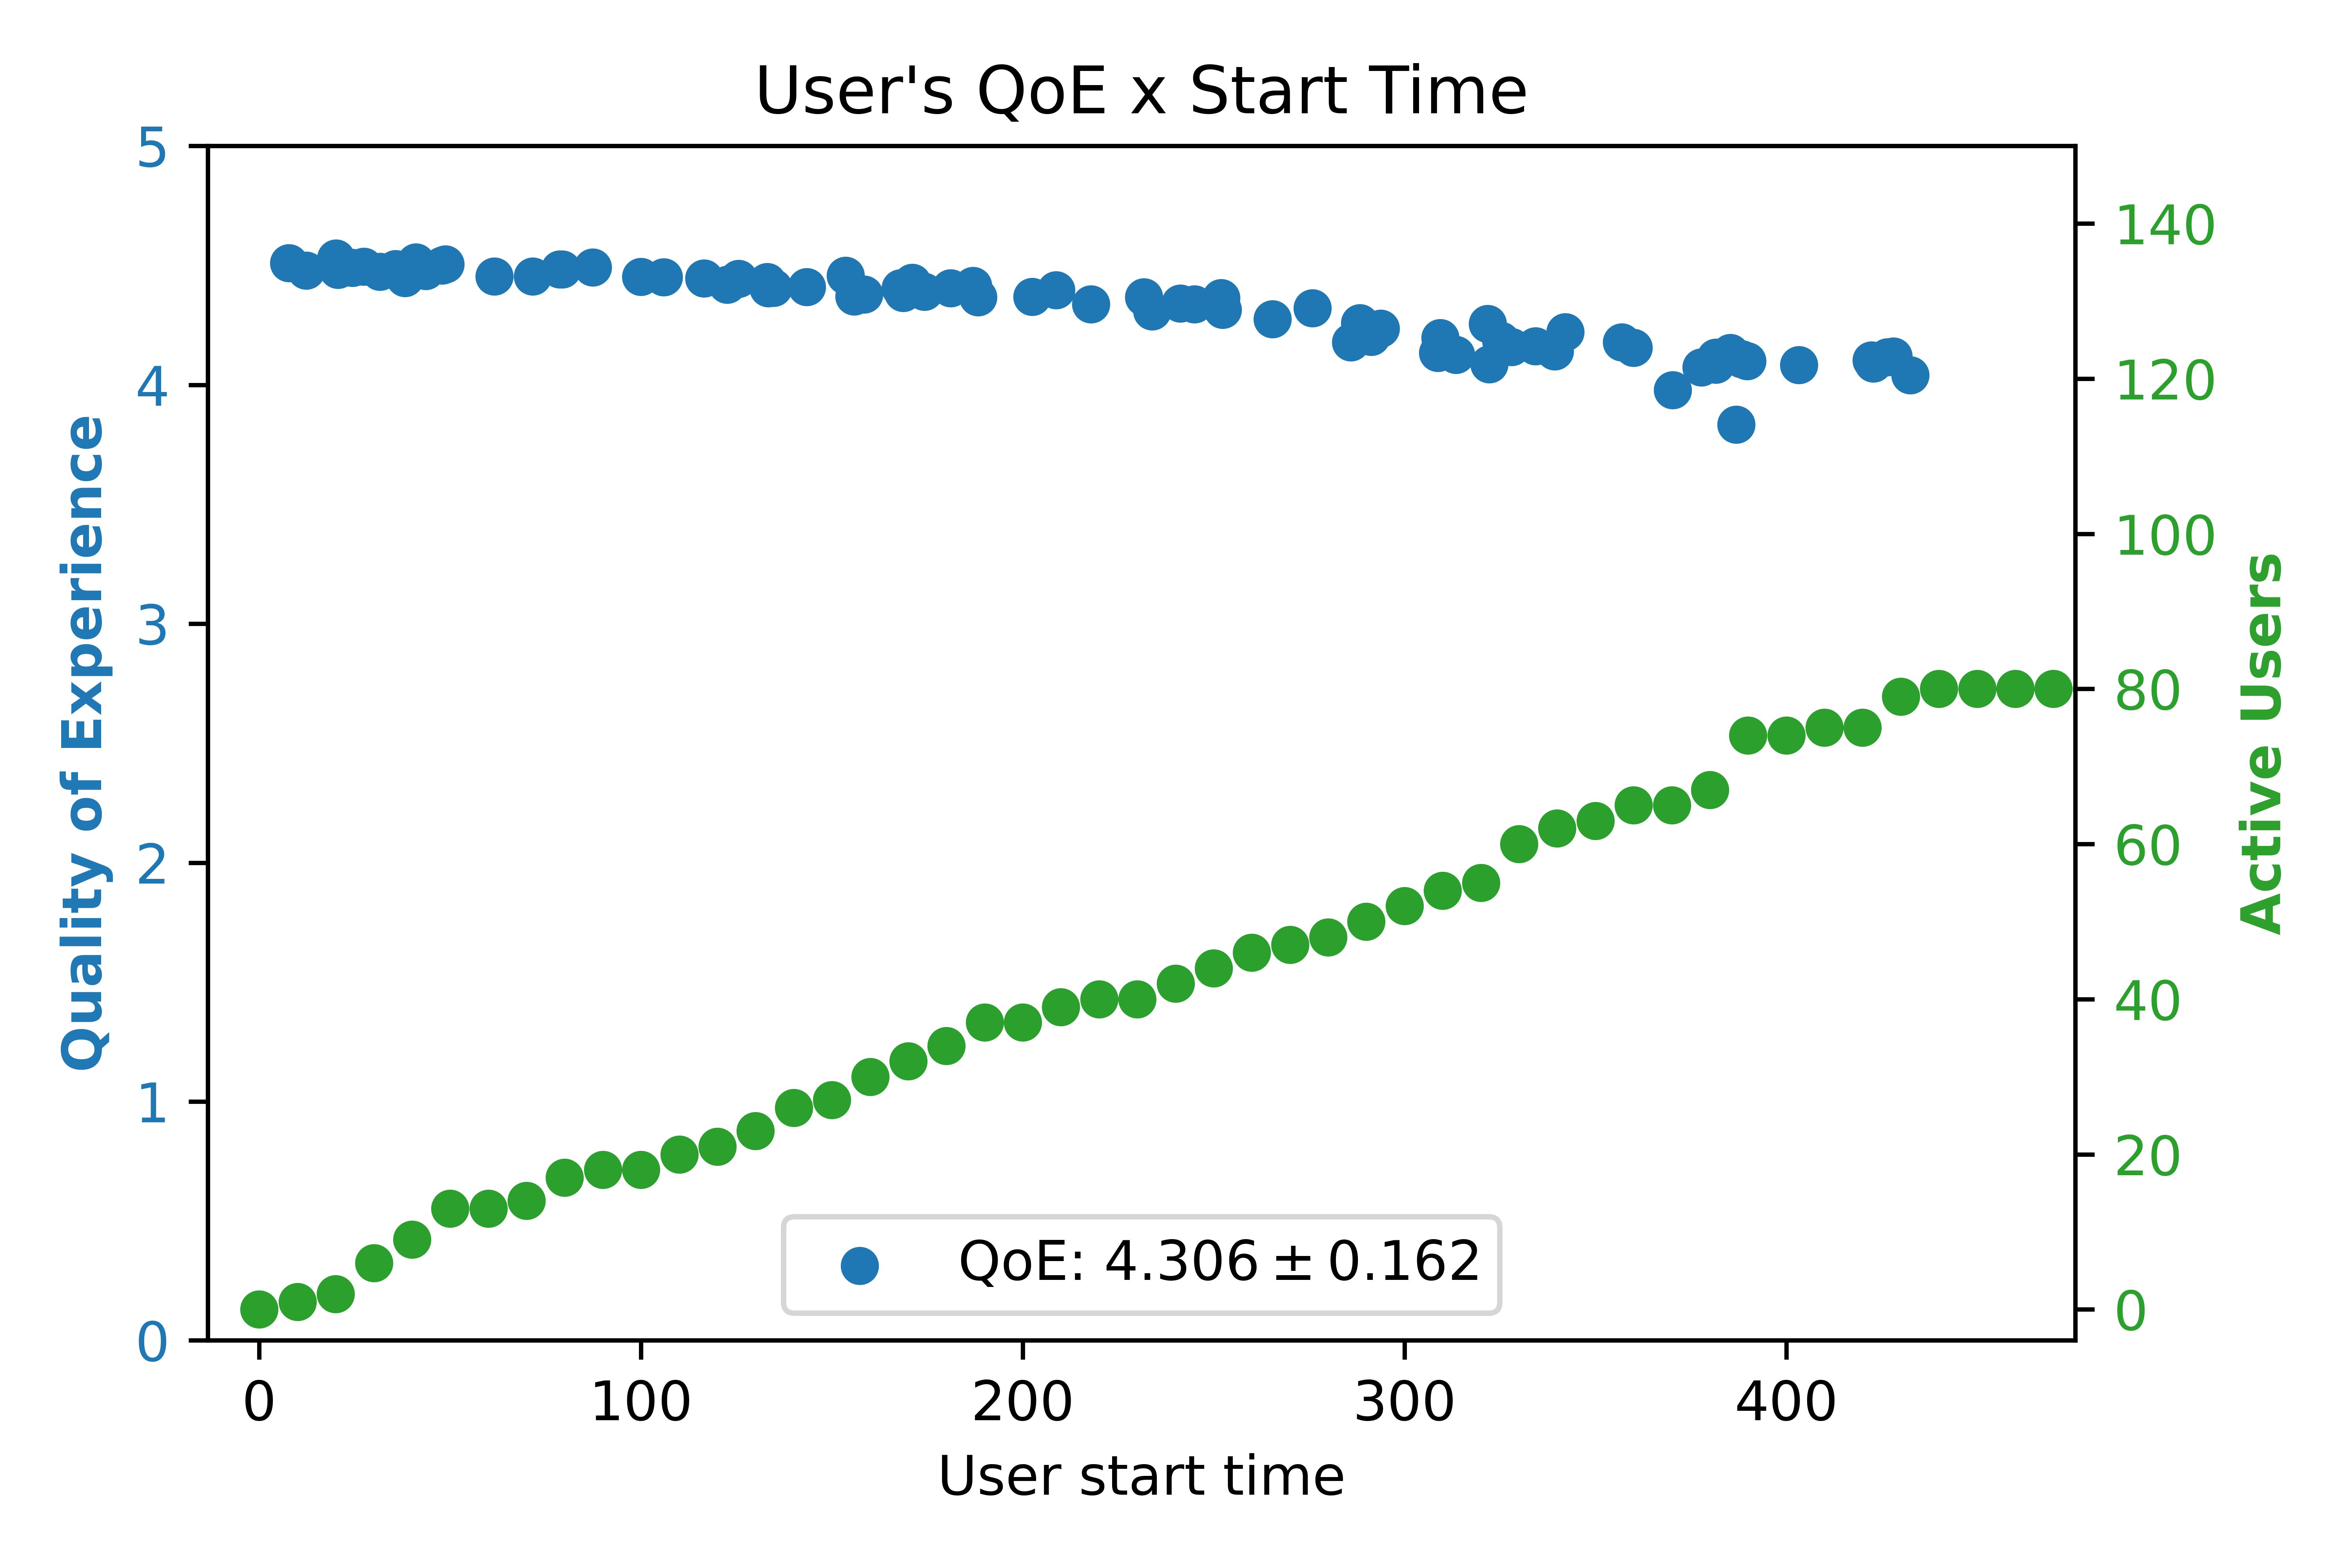
\includegraphics[width=0.31\linewidth]{images/Redicrect_QoExStartTime20.png}
    \label{fig:plr-comparison-2}
    }
    \subfigure[]{
    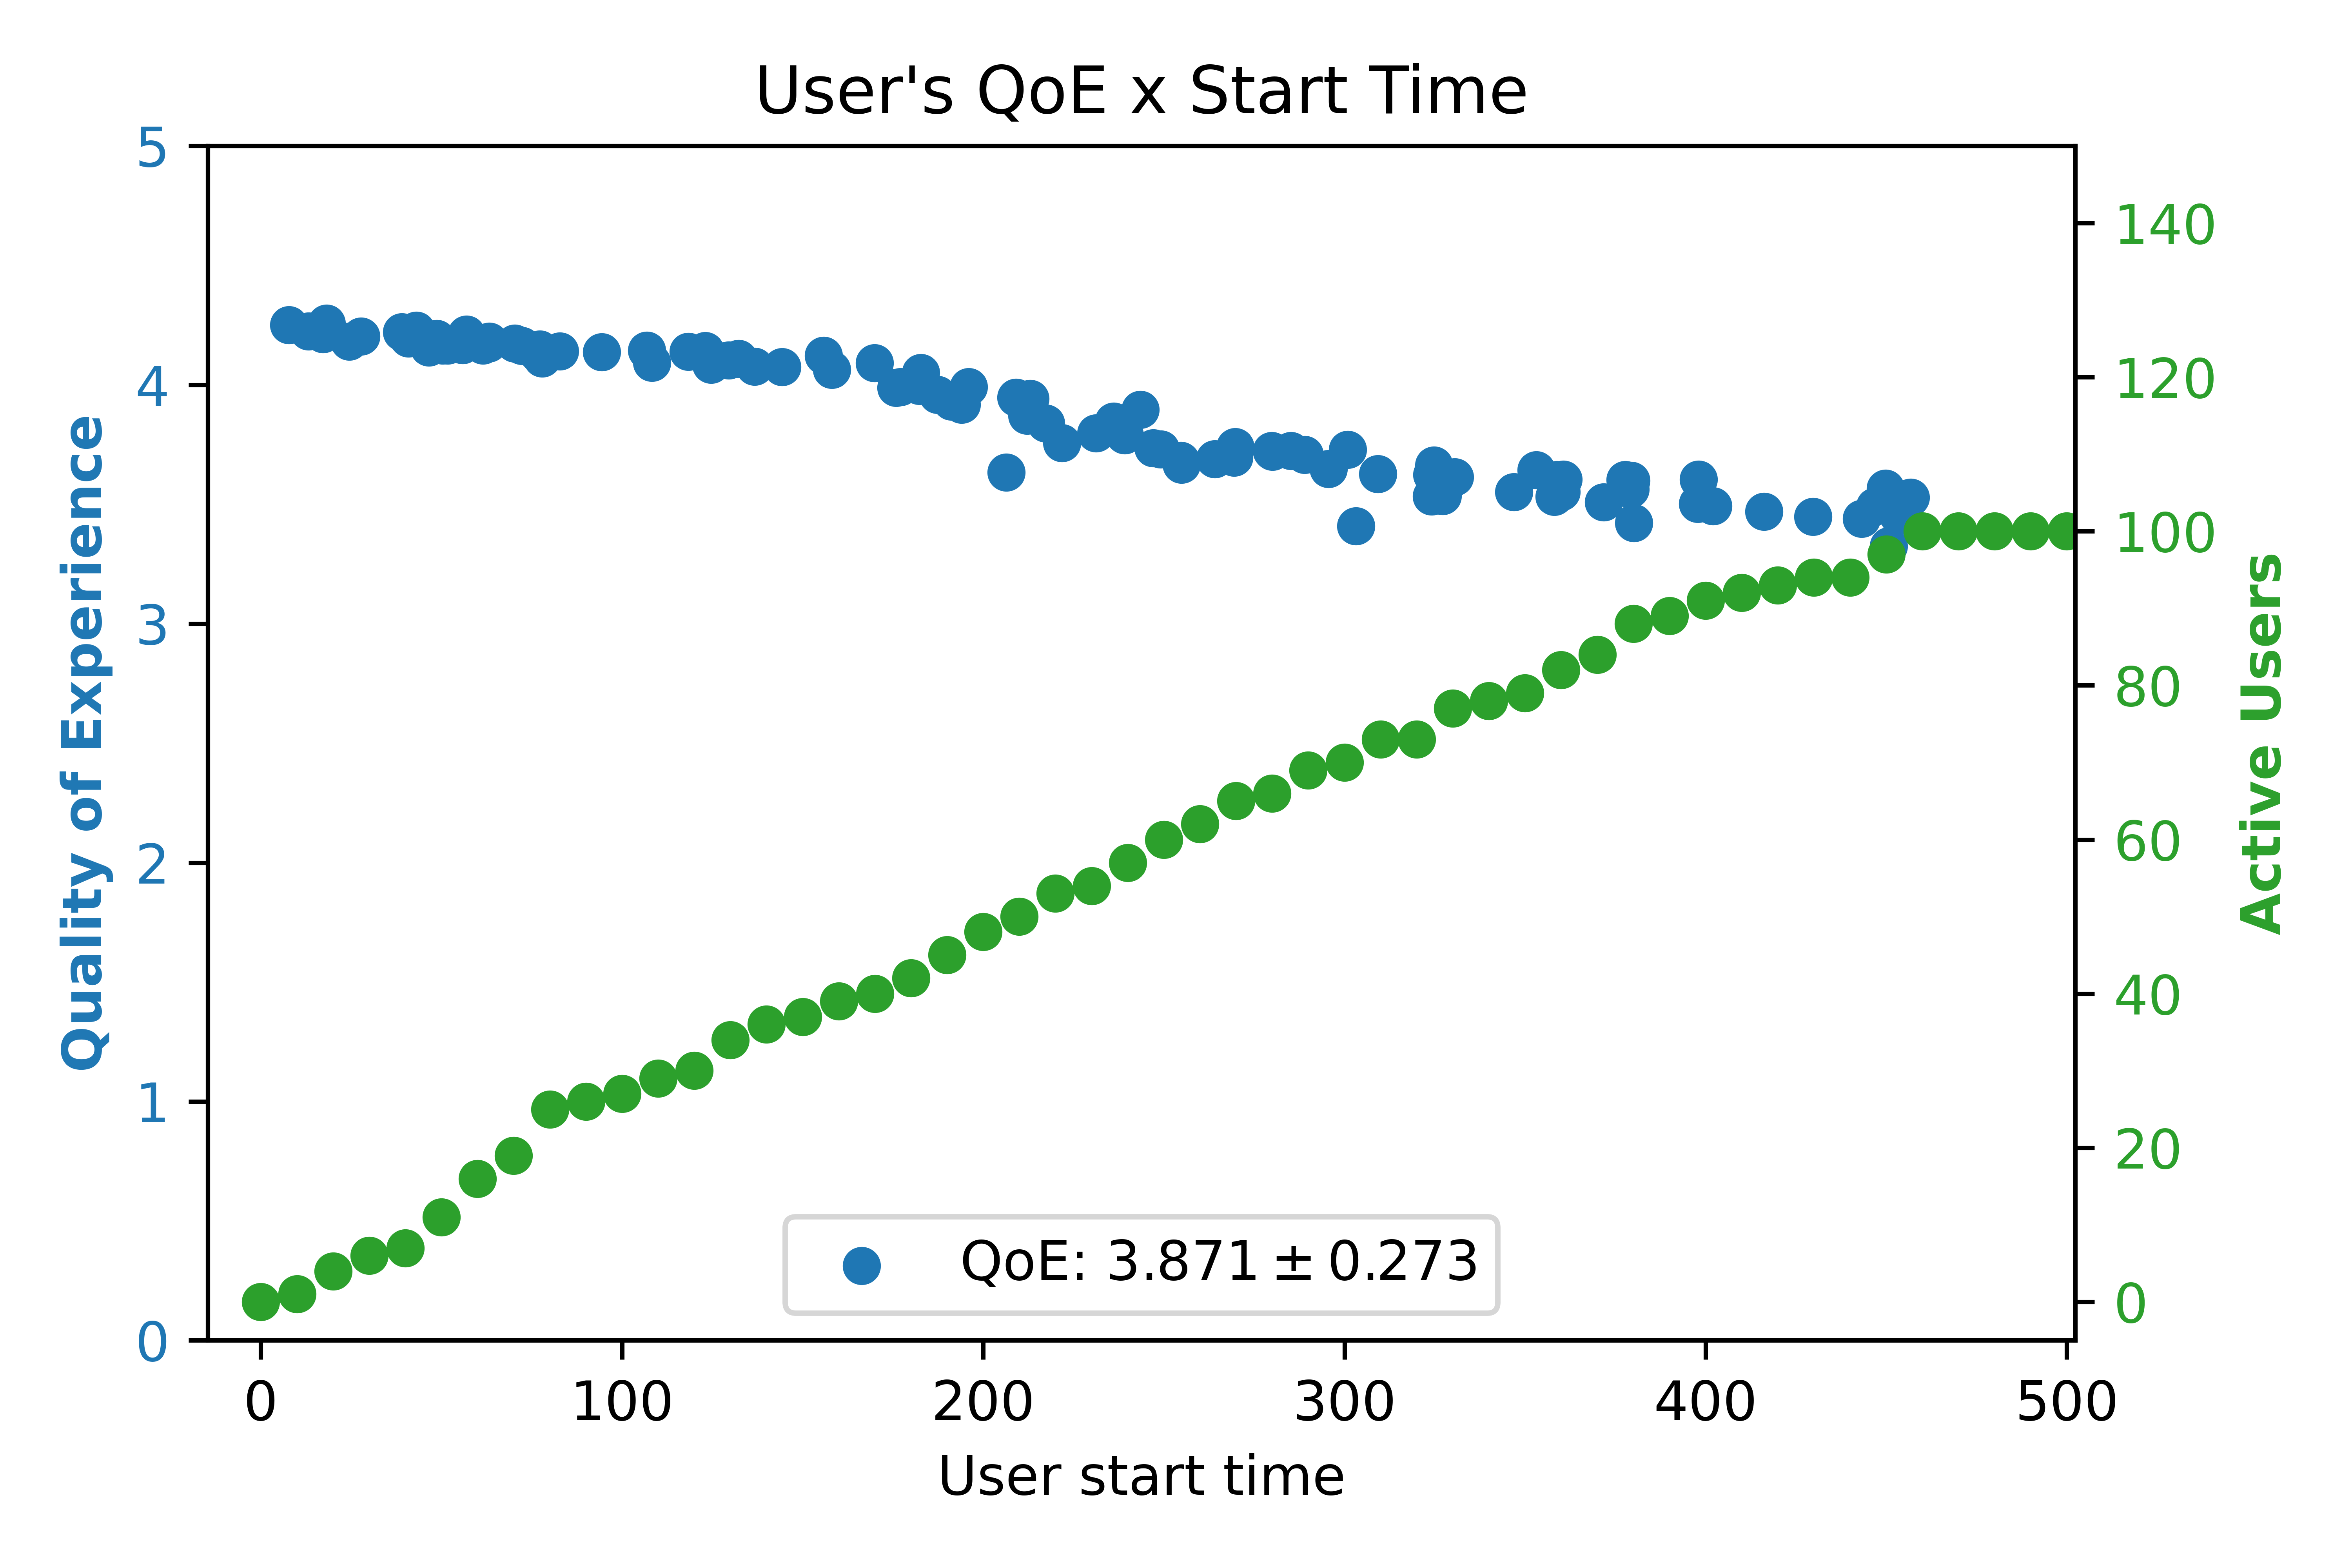
\includegraphics[width=0.31\linewidth]{images/Redicrect_QoExStartTime25.png}
    \label{fig:plr-comparison-2}
    }
    
    \caption{Impact of system on the network performance. Distance \textit{d} between sensor node and antennas of 8m in a semi-NLOS scenario.}
    \label{fig:comparison-qoe-2}
\end{figure*}

\subsection{Results}

We made the experiment illustrated in Figure~\ref{fig:red-comparison-plot} to show the average QoE as shown in~\ref{qoe-equation} to 15, 20 and 25 users. In this experiment, as users reach the final QoE, it tends to be a little lower than the previous one. When looking at the final QoE delta between users $u_{i}$ and $u_{i + 1}$ seem to be irrelevant, but as we increase the delta the QoE starts to become considerable. Through the figure~\ref{fig:co-comparison-boxplot} we can also affirm this behavior, as the number of users increases, the average QoE decreases and the variation between users increases. Also note that the simulation with 25 users per system the system already shows a degradation in the quality perceived by the end user in a negative way.

While Figures~\ref{fig:red-comparison-plot} and~\ref{fig:red-comparison-boxplot} show that a simple video allocation strategy at the edge can help improve the quality of the user experience.

The Figures~\ref{fig:comparison-qoe-2} shows a simple strategy of moving the video to the edge can significantly improve the user's QoE. In this way, the video transmission system is able to provide user satisfaction qualities as well as they tend to keep them watching the video until the end. 

It is important to note that, although the bit rates between the ABR mechanisms are similar, the interruptions they can generate are significantly different, which directly impacts users' QoE. Another point to be noted is the average bit rate between different levels. In the scenario with 20 users, level 3 was able to achieve what is necessary to obtain the highest bit rate representation, thus, network operators can seek to deploy caches during peak hours to provide the best user experience.